\chapter{The logic of sub-intervals $\D$}\label{chap:ICALP}
\begin{chapref}
The reference for this chapter is \cite{icalp17}.
\end{chapref}

\minitoc\mtcskip

\newcommand{\CL}{\mathsf{CL}}
\newcommand{\REQ}{\mathsf{REQ}}
\newcommand{\obsD}{\cO bs_D}
\newcommand{\reqD}{\cR eq_D}
\newcommand{\rank}{rank}
\newcommand{\row}{row}
\newcommand{\orow}{\overline{row}}
\newcommand{\Atoms}{\cA_{\varphi}}
\newcommand{\Rows}{\cR ows_{\varphi}}

\newcommand{\bbD}{\mathbb{S}}
\newcommand{\bbI}{\mathbb{I}}
\newcommand{\bbP}{\mathbb{P}}

\newcommand{\cA}{\mathcal{A}}
\newcommand{\cG}{\mathcal{G}}
\newcommand{\cH}{\mathcal{H}}
\newcommand{\cL}{\mathcal{L}}
\newcommand{\cO}{\mathcal{O}}
\newcommand{\cR}{\mathcal{R}}
\newcommand{\cV}{\mathpzc{V}}
\newcommand{\hA}{\hat{A}}
\newcommand{\hn}{\hat{n}}
\newcommand{\hm}{\hat{m}}

\newcommand{\om}{\overline{m}}

\newcommand{\bM}{\mathbf{M}}

\newcommand{\subint}{\sqsubset}
\newcommand{\subinteq}{\sqsubseteq}
\newcommand{\ssubint}{{\text{$\sqsubset$\llap{$\;\cdot\;$}}}}
\newcommand{\Dphi}{\mathrel{D_\varphi}}
\newcommand{\Dref}{\textsf{D$_\subinteq$}\xspace}
\newcommand{\Dirr}{\textsf{D$_\subint$}\xspace}
\newcommand{\Dstr}{\textsf{D$_\ssubint$}\xspace}
\newcommand{\Dsim}{\textsf{D$_\circ$}\xspace}


\newcommand{\genDphi}{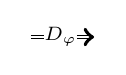
\begin{tikzpicture}
\node(A)[inner sep=0pt]{$\scriptstyle\Dphi$};
\node[inner sep=0pt](B) at (0.45,0){};
\node[inner sep=0pt](C) at (-0.4,0){};
\draw[double](C) -- (A);
 \draw[double,->](A) --(B); 
\end{tikzpicture}}

\newcommand{\rownext}{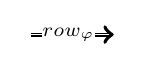
\begin{tikzpicture}
\node(A)[inner sep=0pt]{$\scriptstyle row_{\varphi}$};
\node[inner sep=0pt](B) at (0.6,0){};
\node[inner sep=0pt](C) at (-0.5,0){};
\draw[double](C) -- (A);
 \draw[double,->](A) --(B); 
\end{tikzpicture}}

\newcommand{\genDphiS}{\begin{tikzpicture}
\node(A)[inner sep=0pt]{$\scriptstyle{\Dphi\ssubint}$};
\node[inner sep=0pt](B) at (0.7,0){};
\node[inner sep=0pt](C) at (-0.6,0){};
\draw[double](C) -- (A);
\draw[double,->](A) --(B); 
\end{tikzpicture}}

\newcommand{\rownextS}{\begin{tikzpicture}
\node(A)[inner sep=0pt]{$\scriptstyle row_{\varphi}\ssubint$};
\node[inner sep=0pt](B) at (0.8,0){};
\node[inner sep=0pt](C) at (-0.7,0){};
\draw[double](C) -- (A);
\draw[double,->](A) --(B); 
\end{tikzpicture}}

\newcommand{\hsDhom}{\D}%{\textup{D}$|_{\cH om}$}


\lettrine[lines=3]{A}{\ good balancing} of \emph{expressiveness} and \emph{complexity} in the choice 
of the system 
model and of the specification language is a key factor for the effective 
exploitation of MC. 
Various improvements to both of them have been proposed in the literature. As 
for the latter we recall in particular the extensions of $\LTL$ with 
promptness, that make it 
possible to bound the delay with which a liveness request is fulfilled (see, 
e.g.,~\cite{DBLP:journals/fmsd/KupfermanPV09}). 
Another possible direction is
\emph{adding regular expressions}, that allow one to enrich the expressive 
power of existing logics. This has been investigated, for instance, in the 
cases of $\LTL$~\cite{Leucker2007} and $\CTL$~\cite{MATEESCU20112854}.
%
In this chapter, we study the MC problem for \emph{$\HS$ extended with regular 
expressions}, which are exploited as a means for \emph{relaxing the homogeneity 
assumption}, that otherwise limits the expressive power of $\HS$. 

As we have already said (Section~\ref{sec:LOMrelated}), in~\cite{lm16} %the first meaningful attempt to relax the homogeneity assumption can be found, where 
Lomuscio and Michaliszyn propose to use regular expressions to define the 
labeling of proposition letters over intervals in terms of the component 
states---thus relaxing homogeneity, that can be trivially \lq\lq 
encoded\rq\rq{} by regular expressions, as shown later. In that work the 
authors prove decidability of MC with regular expressions for some very 
restricted fragments of epistemic $\HS$, giving some rough upper bounds to its 
computational complexity
(see the fourth column of Table~\ref{fig:overv}).
%
In this chapter, 
we define interval labeling via regular expressions in a way that 
can be shown to be equivalent to that of~\cite{lm16}, and
we give a detailed picture of decidability and complexity for $\HS$ with 
regular expressions, which was still missing. The results are summarized in the 
third column of Table~\ref{fig:overv}. 

\begin{table}
	\centering
	\caption{Complexity of MC for $\HS$ and its fragments ($^\dagger$local MC). 
	In red, the new results proved in this chapter.}\label{fig:overv}
	\resizebox{\textwidth}{!}{
		\begingroup
\renewcommand*{\arraystretch}{1.3}
%
\begin{tabular}{|@{\ }c@{\ }|@{\ }c@{\ }|@{\ }c@{\ }||@{\ }c@{\ }|}
\hline 
 & Homogeneity & Regular expressions & Endpoints~\cite{LM13,LM14,lm16}\\
\hline \hline 
\multirow{2}{*}{Full $\HS$, $\B\E$} & nonelementary  & \textcolor{red}{nonelementary}  & $\B\E$+$\epist^\dagger$: $\Psp$ \\
%\cline{2-4} 
 & $\EXPSPACE$-hard & $\EXPSPACE$-hard & $\B\E^\dagger$: $\PTIME$\\
\hline 
\multirow{2}{*}{$\A\Abar\B\Bbar\Ebar,\A\Abar\E\Bbar\Ebar$} & $\in\EXPSPACE$ \textcolor{red}{$\in\LINAEXPTIME$}& nonelem.\  $\Psp$-hard &\\
%\cline{2-4} 
 & $\Psp$-hard & \textcolor{red}{$\LINAEXPTIME$-complete}& \\
\hline 
\multirow{2}{*}{$\AAbar\Bbar\Ebar$} & \multirow{2}{*}{$\Psp$-complete} & \textcolor{red}{$\in\LINAEXPTIME$} & \\
 & & $\Psp$-hard & \\
\hline
$\AAbarBBbar,\B\Bbar,\Bbar,$ & \multirow{2}{*}{$\Psp$-complete} & \multirow{2}{*}{\textcolor{red}{$\Psp$-complete}} & \multirow{2}{*}{$\A\Bbar$+$\epist$: nonelementary}\\
$\AAbarEEbar,\E\Ebar,\Ebar$ & & & \\
\hline 
$\AAbar\B,\AAbar\E,\A\B,\Abar\E$ & $\PTIME^{\NP}\!$-complete & \textcolor{red}{$\Psp$-complete} & \\
\hline 
\multirow{2}{*}{$\A\Abar,\Abar\B,\A\E,\A,\Abar$} & $\in\Thsq$ & \multirow{2}{*}{\textcolor{red}{$\Psp$-complete}} & \\
%\cline{2-2} \cline{4-4} 
 & $\Th$-hard &  & \\
\hline 
$\HSprop, \B,\E$ & $\co\NP$-complete & \textcolor{red}{$\Psp$-complete} & \\
\hline 
\end{tabular}

\endgroup
	}
	%\vspace*{-0.2cm}
\end{table}

It is interesting to compare the complexity of MC for $\HS$ fragments extended with regular expressions with the same fragments under the homogeneity assumption. The rich spectrum of complexities for the less expressive fragments of $\HS$ under homogeneity (last four rows in the table) collapses to $\Psp$-completeness in the case of the corresponding fragments with regular expressions, witnessing that using regular expressions increases the expressive power of (syntactically) small fragments of $\HS$. Whether or not there exists an elementary algorithm for full $\HS$ remains an open issue, just like in the case of full $\HS$ under homogeneity. The main results of the chapter are summarized in the following account of the contents of the next sections.

\paragraph*{Organization of the chapter.}
\begin{itemize}

\item
In Section~\ref{sect:backgrRegex}, we start by recalling the notions of regular expression and finite-state automaton, and then give syntax and semantics of $\HS$ with regular expressions.

\item
In Section \ref{sect:fullHS}, we prove that MC for (full) $\HS$ extended with regular expressions (under the state-based semantics) is decidable,
by exploiting an automata-theoretic approach and the notion of $\Ku$-\NFA, a particular version of finite-state automaton. 
Moreover, the problem can be shown to be in $\PTIME$ when it is restricted to 
system models, assuming the formula to be of constant length. 

\item
Then, in Section~\ref{sec:AAbarBBbarEbarRegex},
we study the problems of MC for the two (syntactically) maximal (symmetric) 
fragments $\A\Abar\B\Bbar\Ebar$ and $\A\Abar\E\Bbar\Ebar$ with regular 
expressions, proving that both problems are $\LINAEXPTIME$-complete. 
$\LINAEXPTIME$ denotes the complexity class of problems decided by   
\emph{exponential-time bounded} alternating Turing machines making a 
\emph{polynomially 
bounded number of alternations}; such a class captures the exact complexity of 
some relevant problems~\cite{tcs15l,FR75}, such as, for instance, the 
first-order 
theory of real addition with order~\cite{FR75}.
First, we recall (Chapter~\ref{chap:TCS17}) that settling the exact complexity 
of these fragments under the homogeneity assumption is a difficult open 
question. Moreover,  considering that $\LINAEXPTIME \subseteq \AEXP = \EXPSPACE$ and 
that $\HS$ under homogeneity  is subsumed by $\HS$ with regular expressions (as 
we will see later), 
the results proved in this chapter improve  the complexity upper bounds for the 
fragments  
$\A\Abar\B\Bbar\Ebar$ and $\A\Abar\E\Bbar\Ebar$ given in 
Section~\ref{sec:AAbarBBbarEbar}. 
%
More in detail, we preliminarily establish an exponential small-model property 
for $\A\Abar\B\Bbar\Ebar$ (Section~\ref{sec:AAbarBBbarEbarTrackProperty}): for 
each interval (trace),  it is possible to find an interval of bounded 
exponential 
length that is indistinguishable with respect to the fulfillment of 
$\A\Abar\B\Bbar\Ebar$ formulas (respectively, $\A\Abar\E\Bbar\Ebar$ formulas).
Such a property allows us to devise an MC procedure belonging to the class $\LINAEXPTIME$ (Section~\ref{sec:UpperBound}). 
Finally, the %hardness of the problem 
matching lower bounds are obtained % proved for the fragment $\B\Ebar$ of $\A\Abar\B\Bbar\Ebar$ 
by polynomial-time reductions from the so-called \emph{alternating multi-tiling 
problem}, showing that they already hold for the fragments $\B\Ebar$ and 
$\E\Bbar$ of $\A\Abar\B\Bbar\Ebar$ and $\A\Abar\E\Bbar\Ebar$, respectively 
(Section~\ref{sec:LowerBound}). 

\item
Finally, in Section~\ref{sec:AABB}, we show that 
formulas of $\HS$ fragments featuring (any subset of) $\HS$ modalities for the Allen's relations \emph{meets, met-by, started-by}, and \emph{starts} ($\AAbarBBbar$) can be checked in polynomial working space (MC for all these is $\Psp$-complete). 
%
In particular, in Section~\ref{subsec:AAbarEEbar} we prove a small-model 
theorem for $\AAbarBBbar$ (and the symmetric $\AAbarEEbar$) with regular 
expressions, which is then 
exploited in Sections~\ref{sect:PspAlgo} and \ref{sect:genResult} to devise a 
$\Psp$ MC algorithm for $\AAbarBBbar$ (and $\AAbarEEbar$). Moreover, in 
Section~\ref{sect:genResult}, we prove that MC for the purely propositional 
fragment of $\HS$, denoted as $\HSprop$, is hard for $\Psp$, which is enough to 
conclude that MC for any sub-fragment of $\AAbarBBbar$ or $\AAbarEEbar$ is 
complete for $\Psp$.
%
Hence, relaxing the homogeneity assumption via regular expressions comes at no 
cost for $\AAbarBBbar$, $\AAbarEEbar$, $\B\Bbar$, $\E\Ebar$, $\Bbar$ and 
$\Ebar$---that remain in $\Psp$---while $\AAbarB$ and $\A\Abar\E$ and their 
sub-fragments
%$\B$, $\E$, $\AAbar$, $\AAbarB$, $\A\Abar\E$, \dots{} 
increase their complexity to $\Psp$ (see Table~\ref{fig:overv} once more). 
\end{itemize}
\section{Preliminaries}\label{sec:preliminaries}

To start with, we introduce some preliminary notions.
Let $\mathbb{S} = (\mathpzc{S}, <)$ be a  linear order. An
\emph{interval} over $\mathbb{S}$ is an ordered pair $[x, y]$,
where $x,y\in \mathpzc{S},\, x \leq y$, representing the set $\{z\in \mathpzc{S}\mid x\leq z\leq y\}$. We denote the set of all intervals over
$\mathbb{S}$ by $\mathbb{I(S)}$.
%
We consider three possible \emph{sub-interval relations}: 
\begin{enumerate}
    \item the \emph{reflexive} sub-interval relation (denoted as
    $\sqsubseteq$), defined by $[x, y] \sqsubseteq [x', y']$ if and only if
    $x' \leq x$ and $y\leq y'$,
    % 
    \item the \emph{proper (or
    irreflexive)} sub-interval relation (denoted as $\subint$), defined
    by $[x, y]\subint  [x', y']$ if and only if $[x, y] \sqsubseteq
    [x', y']$ and $[x, y] \neq [x', y']$, and 
    %
    \item the \emph{strict}
    sub-interval relation (denoted as $\ssubint$), defined by 
    $[x, y] \ssubint [x', y'] $ if and only if $x' < x$ and $y<y'$.
\end{enumerate}

The three modal logics $\Dref$, $\Dirr$, and $\Dstr$ feature the same
language, consisting of a set $\AP$ of proposition
letters, the logical connectives $\neg$ and $\vee$, and the
modal operator $\hsD$. Formally, formulas are
defined by the grammar: \[\varphi ::= p \ |\ \neg\varphi\ |\ \varphi \vee \varphi\ |\ \hsD \varphi,\]
%\[
%\varphi ::= p \ |\ \neg\varphi\ |\ \varphi \vee \varphi\ |\ \D \varphi ,
%\]
with $p\in\AP$.
The other connectives, as well as
the logical constants $\top$ (true) and $\bot$ (false), are defined as usual; moreover, the
dual universal modal operator $\hsDu\varphi$ is defined as $\neg\hsD\neg\varphi$. The length of a formula
$\varphi$, denoted as $|\varphi|$, is the number of subformulas of $\varphi$.

The semantics of~\Dstr, \Dirr, and \Dref only differ in the
interpretation of the $\hsD$ operator. For the sake of brevity, we use
$\circ \in \{\ssubint,\subint,\subinteq \}$ as a shorthand for
any of the three sub-interval relations. The semantics of a
sub-interval logic \Dsim is defined in terms of \emph{interval models}\footnote{Not to be confused with the previously introduced \emph{abstract interval models}.}
$\bM=(\mathbb{I(S)},\circ,\cV)$. The \emph{valuation
function} $\cV : \AP \to 2^{\mathbb{I(S)}}$ assigns to
every proposition letter $p$ the set of intervals $\cV(p)$ over
which $p$ holds. The \emph{satisfiability relation} $\models$ is
defined as:
%
\begin{itemize}
  \item for every proposition letter  $p \in \AP$, $\bM, [x,y]
        \models p$ if and only if $[x,y] \in \cV(p)$;

  \item $\bM, [x,y] \!\models\! \neg \psi$ if and only if $\bM, [x,y]
        \!\not\models\! \psi$ (i.e. it is not true that $\bM, [x,y]
        \!\models\! \psi$);

  \item $\bM, [x,y] \models \psi_1 \vee \psi_2$ if and only if $\bM, [x,y] \models \psi_1$ or $\bM, [x,y] \models \psi_2$;

  \item $\bM, [x,y] \models \hsD \psi$ if and only if there exists an interval $[x',y'] \in
        \bbI(\mathbb{S})$ such that $[x',y'] \circ [x,y]$ and
        $\bM, [x',y'] \models \psi$.
\end{itemize}
%
A \Dsim formula is \emph{satisfiable} if it holds over some interval of an interval model, and \emph{valid} if it holds over every interval of every interval model.

As we mentioned earlier on, it can be shown that the logic $\Dref$ turns out to be equivalent to the standard modal logic S4 \cite{DBLP:journals/jphil/Benthem91}. 
%The decidability of the satisfiability problem for the considered logics 
%\Dsim has been widely studied by restricting the class of linear orders to the dense ones 
%\cite{DBLP:journals/corr/MontanariPS15} and to the finite ones 
%\cite{DBLP:journals/fuin/MarcinkowskiM14}. 
%
Here we restrict our attention to the finite SAT problem, that is, satisfiability over the class of finite linear orders. The problem has been shown to be \emph{undecidable} for $\Dirr$ and $\Dstr$~\cite{DBLP:journals/fuin/MarcinkowskiM14} and \emph{decidable} for $\Dref$~\cite{DBLP:conf/time/MontanariPS10}. In the following, we prove that decidability can be recovered for $\Dirr$ and $\Dstr$ by restricting to the class of \emph{homogeneous} interval models. We fully work out the case of $\Dirr$ (for the sake of simplicity, we will write $\D$\ for $\Dirr$), and then we briefly explain how to adapt the proofs to $\Dstr$. 

\begin{definition}\label{def:homogeneous_models}
An interval model
$\bM=(\mathbb{I(S)},\circ,\cV)$ is \emph{homogeneous} if,
for every interval $[x,y]  \in \mathbb{I(S)}$ and every proposition letter $p \in \AP$,
it holds that $[x,y] \in \cV(p)$ if and only if $[x',x'] \in \cV(p)$
for every $x\leq x'\leq y$.
\end{definition}
% 
Hereafter we will assume the logic $\D$ to be interpreted over homogeneous interval models.

\section{A spatial representation of interval models}\label{sec:compass}

Let us now introduce some basic definitions and notation which will be
extensively used in the following, concluding the section with the notion of compass structure. Given a $\D$ formula $\varphi$,
we define the \emph{closure of $\varphi$}, denoted by
$\CL(\varphi)$, as the set of all subformulas $\psi$ of $\varphi$ and of their
negations $\neg\psi$ (we identify $\neg\neg \psi$ with $\psi$). %Moreover we define the notion of $\varphi$-atom as follows.

\begin{definition}\label{def:d-atom}
Given a $\D$-formula $\varphi$, a $\varphi$-atom $A$ is a subset of
$\CL(\varphi)$ such that: 
\begin{itemize}
    \item  for every $\psi \in \CL(\varphi)$, $\psi \in A$ if and only if $\neg\psi \notin A$, and
    \item for every $\psi_1 \vee \psi_2 \in \CL(\varphi)$, $\psi_1 \vee \psi_2 \in A$ if and only if $\psi_1 \in A$ or $\psi_2 \in A$.
\end{itemize}
\end{definition}

The idea underlying atoms is to enforce a \lq\lq local\rq\rq{} (or Boolean) form of consistency among the formulas it contains, that is, a $\varphi$-atom $A$ is a \emph{maximal, locally consistent subset} of $\CL(\varphi)$. As an example, $\neg(\psi_1 \vee \psi_2) \in A$ if and only if $\neg\psi_1\in A$ and $\neg\psi_2\in A$. However, note that the definition does not set any constraint on $\hsD\psi$ formulas, hence the word ``local''.
We denote the set of all $\varphi$-atoms as $\cA_\varphi$; its cardinality is clearly bounded by $2^{|\varphi|}$ (by the first point of Definition~\ref{def:d-atom}). Atoms are connected by the following binary relation $\Dphi$.

\begin{definition}\label{def:Dphi-relation}
Let $\Dphi$ be a binary relation over $\cA_\varphi$ such that, for each pair of atoms $A, A' \in \cA_\varphi$, $A \Dphi A'$ holds if and only if both $\psi \in A'$ and $\hsDu\psi \in A'$ for each formula $\hsDu\psi \in A$.
\end{definition}

Let $A$ be a $\varphi$-atom. We denote by $\reqD(A)$ the set $\{\psi \in \CL(\varphi) \mid \hsD \psi \in A\}$ of \lq\lq \emph{temporal requests}\rq\rq{} of $A$. In particular, if $ \psi \notin \reqD(A)$, then $\hsDu \neg \psi \in A$ (by the definition of $\varphi$-atom). Moreover, we denote by $\REQ_{\varphi}$ the set of all  arguments of $\D$ formulas in $\CL(\varphi)$, namely, $\REQ_{\varphi}=\{ \psi \mid \hsD \psi\in \CL(\varphi)\}$. Finally, we denote by $\obsD(A)$ the set $\{\psi \in A \mid \psi \in \REQ_{\varphi}\}$ of \lq\lq \emph{observables}\rq\rq{} of $A$. 

It is easy to prove by induction the next proposition stating that, once the proposition letters of $A$ and its temporal requests are fixed, $A$ is determined.
\begin{proposition}\label{prop:unique}
    For any $\D$ formula $\varphi$,
    given a set $R \subseteq \REQ_{\varphi}$ and a set $P \subseteq \CL(\varphi)\cap \AP$, there exists a unique $\varphi$-atom $A$ that satisfies $\reqD(A)=R$ and $A\cap \AP = P$.
\end{proposition} 

We now provide a natural interpretation of $\D$\ over grid-like
structures, called \emph{compass structures}, by exploiting the existence
of a natural bijection between intervals $[x,y]$ and 
points $(x,y)$, with $x \leq y$, of an $\mathpzc{S}\times \mathpzc{S}$ grid, where $\mathbb{S} = (\mathpzc{S},<)$ is a finite linear order. Such an interpretation was originally proposed by Venema in~\cite{venema1990},
and it can also be given for $\HS$ and all its (other) fragments.


\begin{figure}[tb]
%\vspace*{-0.6cm}
\centering
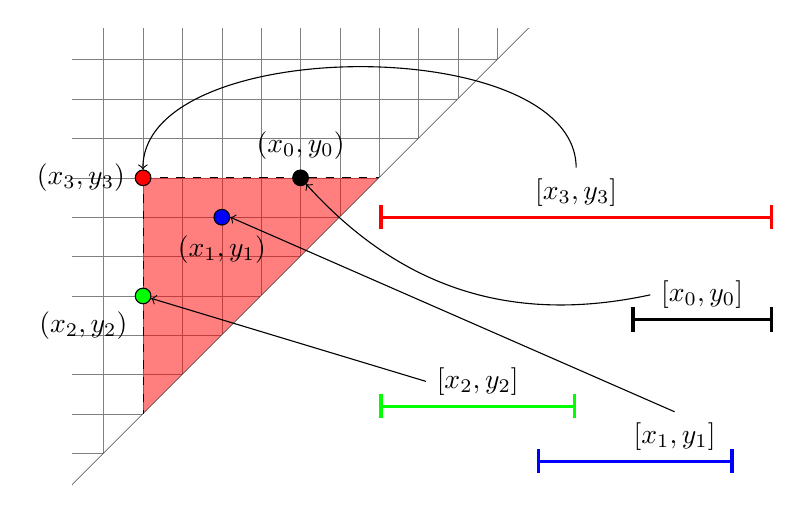
\begin{tikzpicture}[scale=1]

\draw[step=0.5cm,gray,very thin] (-2.9,-2.9) grid (2.9,2.9);
\fill[color=red, opacity=.5] (-2,1) -- (1,1)-- (-2,-2);
\draw (-2.9,-2.9) -- (2.9,2.9);
\fill[color=white] (-2.9,-2.9) -- (2.9,2.9) -- (2.9,-2.9);
\draw[dashed] (-2,1) -- (-2, -2);
\draw[dashed] (-2,1) -- (1, 1);

\node[shape=circle,draw=black,inner sep=2pt,fill=black, label={above :$(x_0,y_0)$}](A) at (0,1) {};

\node[shape=circle,draw=black,inner sep=2pt,fill=red, label={left :$(x_3,y_3)$}](C) at (-2,1) {};

\node[shape=circle,draw=black,inner sep=2pt,fill=blue, label={below :$(x_1,y_1)$}](B) at (-1,0.5) {};
\node[shape=circle,draw=black,inner sep=2pt,fill=green, label={below left:$(x_2,y_2)$}](D) at (-2,-0.5) {};

\pgftransformshift{\pgfpoint{4cm}{-0.5cm}}

\draw[very thick,|-|] (0.2,-0.3) -- (2,-0.3)node[pos=0.5, above](AI) {$[x_0,y_0]$};

\draw(AI.west) edge[->, bend left] (A);

\draw[very thick,|-|,red] (-3,1) -- (2,1)node[pos=0.5, above=0.001cm,black](CI) {$[x_3,y_3]$};

\draw(CI.north) edge[->, bend right=90, looseness=0.8] (C);


\draw[very thick,|-|,blue] (-1,-2.1) -- (1.5,-2.1)node[pos=0.7, above=0.001cm,black](BI) {$[x_1,y_1]$};

\draw(BI.north) edge[->] (B.east);

\draw[very thick,|-|,green] (-3,-1.4) -- (-0.5,-1.4)node[pos=0.5, above=0.001cm,black](DI) {$[x_2,y_2]$};

\draw(DI.west) edge[->] (D);

\end{tikzpicture}
%\vspace*{0.5cm}
\caption{Correspondence between intervals and points of the compass structure.}\label{fig:compassstructure}
%
\end{figure}

As an example, Figure~\ref{fig:compassstructure} shows four intervals
$[x_0,y_0],\ldots,[x_3,y_3]$, respectively represented by the points in the grid $(x_0,y_0),\ldots,(x_3,y_3)$, such that: 
\begin{itemize}
    \item $[x_0,y_0], [x_1,y_1], [x_2,y_2]\subint [x_3,y_3]$, 
    \item $[x_1,y_1] \ssubint [x_3,y_3]$, and 
    \item $[x_0,y_0], [x_2,y_2]\not\!\!\ssubint [x_3,y_3]$. 
\end{itemize}
The red 
region highlighted in Figure~\ref{fig:compassstructure} contains all and only the points $(x,y)$ such that $[x,y]\subint[x_3,y_3]$.
Allen interval relation \emph{contains} can thus be represented as a spatial relation between pairs of points. In the following, we make use of $\subint$ also for relating points, i.e., given two points $(x,y),(x',y')$ of the grid,
$(x',y')\subint (x,y)$ if and only if $(x',y')\neq (x,y)$ and  $x\leq x'\leq y'\leq y$.
%
Compass structures, repeatedly exploited in the following to establish the next complexity results, % as an alternative (and possibly easier to understand) interpretation to linear orders. 
can be formally defined as follows.

\begin{definition}\label{def:compassstructure}
Given a finite linear order $\mathbb{S} = (\mathpzc{S}, <)$ and a $\D$ formula $\varphi$, a  \emph{compass}
$\varphi$-\emph{structure} is a pair $\cG=(\bbP_\bbD,\cL)$,
where $\bbP_\bbD$ is the set of points of the form $(x,y)$,
with $x,y \in \mathpzc{S}$ and $ x\leq y$, and $\cL$ is a function that
maps any point $(x,y)\in\bbP_\bbD$ to a $\varphi$-atom $\cL(x,y)$
in such a way that for every pair of points $(x,y)\neq(x',y')\in\bbP_\bbD$ ,
        if $x\leq x'\leq y'\leq y$ then $\cL(x,y) \Dphi \cL(x',y')$
        (\emph{temporal consistency}).
\end{definition}
%
Due to temporal consistency, the following important property holds in compass structures.
%
\begin{lemma}\label{lem:transitive_req}
Given a compass $\varphi$-structure $\cG=(\bbP_\bbD,\cL)$,
for all pairs of points $(x',y'), (x,y)\in \bbP_\bbD$,
if $(x',y')\subint (x,y)$,
then $\reqD(\cL(x',y')) \subseteq \reqD(\cL(x,y))$ and $\obsD(\cL(x',y')) \subseteq \reqD(\cL(x,y))$.
\end{lemma}
%
\begin{proof} 
%Let us consider a pair of points $(x',y'), (x,y)\in \bbP_\bbD$ such that $(x',y')\subint (x,y)$.
By Definition \ref{def:compassstructure} we have  $\cL(x,y) \Dphi \cL(x',y')$.
Let us assume by contradiction that there exists  $\psi \in \reqD(\cL(x',y'))\setminus \reqD(\cL(x,y))$. By definition of $\reqD$ and by Definition  \ref{def:d-atom}, we have that 
$\psi \in \reqD(\cL(x',y'))$ 
implies   $\hsD\psi \in \cL(x',y')$, and
$\psi \notin \reqD(\cL(x,y))$ 
implies   $\neg\hsD\psi =\hsDu \neg \psi \in \cL(x,y)$. Since $\cL(x,y) \Dphi \cL(x',y')$,
then $\hsDu \neg \psi \in \cL(x',y')$ and thus we can conclude that
both $\hsDu \neg \psi$ and $\hsD \psi$ belong to $\cL(x',y')$ (contradiction).

$\obsD(\cL(x',y')) \subseteq \reqD(\cL(x,y))$ can analogously be proved by contradiction.
\end{proof}

\emph{Fulfilling} compass structures are defined as follows.
%
\begin{definition}\label{def:fulfillingcompass}
%Given a finite linear order $\mathbb{S} = \langle S, <\rangle$, a $\D$-formula $\varphi$ and 
A compass $\varphi$-structure
$\cG=(\bbP_\bbD,\cL)$ is said to be \emph{fulfilling}
if, for every point $(x,y)\in\bbP_\bbD$ and each formula 
$\psi\in \reqD(\cL(x,y))$, 
there exists a point $(x',y')\subint (x,y)$ in $\bbP_\bbD$ such that 
$\psi \in \cL(x',y')$.
\end{definition}
Note that if $\cG$ is fulfilling, then $\reqD(\cL(x,x))=\emptyset$ for all points ``on the diagonal'' $(x,x)\in\bbP_\bbD$.
%
%The following proposition states that satisfiability of a
%$\D$ -formula $\varphi$ is reducible to the problem of deciding whether there exists a fulfilling compass $\varphi$-structure featuring
%$\varphi$.
%
We say that a compass $\varphi$-structure $\cG=(\bbP_\bbD,\cL)$
\emph{features} a formula $\psi$ if there exists a point $(x,y)\in\bbP_\bbD$
such that $\psi \in \cL(x,y)$.
The following result holds.
%
\begin{proposition}\label{prop:compassstructure}
A $\D$ formula $\varphi$ is satisfiable if and only if there exists a fulfilling compass $\varphi$-structure that
features it.
\end{proposition}

In a fulfilling compass $\varphi$-structure  $\cG=(\bbP_\bbD,\cL)$, where $\mathpzc{S}=\{0,\ldots,t\}$, w.l.o.g., we will sometimes assume  $\varphi$ to be satisfied by the maximal interval $[0,t]$, that is, $\varphi\in\cL(0,t)$.%~\cite{sala2010decidability}.

The notion of homogeneous models directly transfers to compass structures.
%
\begin{definition}\label{def:hom_compass}
A compass $\varphi$-structure $\cG=(\bbP_\bbD,\cL)$ is \emph{homogeneous}
if, for every point $(x,y)\in \bbP_\bbD$ and each proposition letter $p\in \AP$,
we have that $p\in \cL(x,y)$ if and only if $p\in \cL(x',x')$ for all $x\leq x'\leq y$.
\end{definition}

Proposition \ref{prop:compassstructure} can be tailored to homogeneous compass structures.
%
\begin{proposition}\label{prop:satiffcompass}
A $\hsDhom$ formula $\varphi$ is satisfiable if and only if there exists a fulfilling homogeneous compass $\varphi$-structure that
features it.
\end{proposition}
\section{SAT of $\hsDhom$\ over finite linear orders}\label{sec:decidability}

In this section, we devise a SAT checking procedure for $\hsDhom$ formulas over finite linear orders, which will also allow us to easily derive a MC algorithm for $\hsDhom${} over finite Kripke structures.

To start with, we show that there is a ternary relation between $\varphi$-atoms, that we denote by $\genDphi$, such that if it holds among all atoms in consecutive positions of a compass $\varphi$-structure, then the structure is fulfilling. Hence, we may say that $\genDphi$ is the rule for labeling fulfilling compasses. 

Next, we introduce an equivalence relation $\sim$ between \emph{rows} of a compass $\varphi$-structure. Since it has finite index---exponentially bounded by $|\varphi|$---and it preserves fulfillment of compasses, it is intuitively possible to ``contract'' the structures when we can find two related rows. Moreover, any contraction done according to $\sim$ keeps the same atoms (only the number of their occurrences may vary), and thus if a compass features $\varphi$ before the contraction, then $\varphi$ is still featured after it. This fact is exploited to build a SAT algorithm for $\hsDhom$ formulas which makes use of \emph{polynomial working space}, because $(i)$~it only needs to keep track of two rows of a compass at a time, $(ii)$~all rows satisfy some nice properties that make it possible to succinctly encode them, and $(iii)$~compass contractions are implicitly performed by means of a reachability check in a suitable graph, whose nodes are the equivalence classes of $\sim$.

Let us now introduce the aforementioned ternary relation $\genDphi$ among atoms.
\begin{definition}\label{def:d_generator}
Given three $\varphi$-atoms $A_1, A_2$ and $A_3$, we say that 
$A_3$ is $\Dphi$-generated by $A_1, A_2$,
written $A_1A_2\genDphi A_3$, if:  
\begin{itemize}
    \item $A_3\cap\AP = A_1 \cap A_2 \cap \AP$ and 
    \item $\reqD(A_3)=\reqD(A_1)\cup \reqD(A_2) \cup \obsD(A_1 )\cup \obsD (A_2)$.
\end{itemize}
\end{definition}


 %We will prove interesting properties related to homogeneous compass structures using  $\genDphi$. First we prove the following little property. 
%
%\begin{lemma}\label{lem:gen_implies_d}
%Given three $\varphi$-atoms $A_1, A_2$ and $A_3$  such that  
%$A_1A_2\genDphi A_3$ then  
%$A_3 \Dphi A_1$ and $A_3\Dphi A_2$.
%\end{lemma}
%\begin{proof}%PROVA OMETTIBILE
%From the definition of $\D\psi$ we have to prove that 
%for every $\BD \psi \in A_3$ we have $\{\BD \psi , \psi\}\in A_1 \cap A_2$.
%Let  $\BD \psi \in A_3$ since  $\BD \psi = \neg \D\neg \psi $
%we have $\neg \psi \notin \reqD(A_3)$. By Definition \ref{def:d_generator} 
%we have $\reqD(A_3)=\reqD(A_1)\cup \reqD(A_2) \cup \obsD(A_1 )\cup \obsD (A_2)$
%and thus $\neg \psi \notin \reqD(A_1)\cup \reqD(A_2) \cup \obsD(A_1 )\cup \obsD (A_2)$
%which means that $\neg \psi \notin \reqD(A_1)\cup \reqD(A_2)$ implies  $\BD \psi \in A_1 \cap A_2$ and $\neg \psi \notin\obsD(A_1 )\cup \obsD (A_2)$
%implies $\psi \in A_1\cap A_2$. We can conclude that $A_3 \Dphi A_1$ and $A_3\Dphi A_2$.
%\end{proof}

It is immediate to show that $A_1A_2\genDphi A_3$ if and only if $A_2A_1\genDphi A_3$ (i.e., the order of the first two components in the ternary relation is irrelevant). 
Notice that the first point of the definition enforces the homogeneity assumption.

The next result, immediately following from Proposition~\ref{prop:unique}, proves that $\genDphi$ expresses a \emph{functional dependency} on $\varphi$-atoms.
%
\begin{lemma}\label{lem:functional}
Given two $\varphi$-atoms $A_1, A_2\in \Atoms$, there exists \emph{exactly one} $\varphi$-atom  $A_3\in \Atoms$  such that $A_1A_2\genDphi A_3$.
\end{lemma}
%
% \begin{proof} 
% Let us suppose by contradiction that there exist $A_3$ and $A_3'$ in $\Atoms$ such that $A_3\neq A_3'$, $A_1A_2\genDphi A_3$ and  $A_1A_2\genDphi A_3'$.
% By Definition \ref{def:d-atom} we  can assume w.l.o.g.\ that there exists $\psi\in \CL(\varphi)$ such that $\psi \in A_3$ and $\neg \psi \in A_3'$.
% Moreover we choose $\psi$ as a minimal formula that satisfies $\psi \in A_3$ and $\neg \psi \in A_3'$, i.e.,
% each proper sub-formula $\psi'$ of $\psi$ either belongs to both $A_3$ and $A_3'$ or does not belong to either 
% $A_3$ or $A_3'$.

% Let us now prove that we get a contradiction.
% If $\psi=p$, with $p\in \AP$, by Definition~\ref{def:d_generator} $A_3\cap\AP = A_1 \cap A_2 \cap \AP $ and thus $p \in A_1\cap A_2\cap \AP $; since $A_3'\cap\AP = A_1 \cap A_2 \cap \AP $,
% we have $p\in A_3'$. Hence, both $p$ and $\neg p$ belong to $A_3'$ which contradicts Definition~\ref{def:d-atom}.

% If $\psi=\neg \psi_1$, by the minimality of $\psi$,
% either $\psi_1\in A_3\cap A_3'$ or $\psi_1\notin A_3\cup A_3'$.
% In the former case we have $\neg \psi_1, \psi_1\in A_3$ (contradiction).
% As for the latter, since we are assuming $\neg \psi\in A_3'$, we have $\neg \neg \psi_1\in A_3'$,
% i.e., $\psi_1\in A_3'$ (contradiction).

% If $\psi= \psi_1 \vee \psi_2 $, let us consider w.l.o.g.\ the case in which 
% $\psi_1 \in A_3$. Since $\neg (\psi_1 \vee \psi_2)\in A_3'$ we have $\neg \psi_1 \in A_3'$
% and thus $\psi_1 \notin A_3'$. However, 
% by the minimality of $\psi$  and since $\psi_1 \in A_3$, we have that 
% $\psi_1\in A_3'$ (contradiction). 

% Finally,
% if $\psi=\D \psi_1$
% then $\neg \D \psi_1 \in A_3'$, hence $\psi_1\notin \reqD(A_3')=\reqD(A_1)\cup \reqD(A_2) \cup \obsD(A_1 )\cup \obsD (A_2)$. Since $\psi \in A_3$ we have $\psi_1\in \reqD(A_3)= \reqD(A_1)\cup \reqD(A_2) \cup \obsD(A_1 )\cup \obsD (A_2)$ (contradiction). 
% \end{proof}

Definition~\ref{def:d_generator} and Lemma~\ref{lem:functional} can be exploited to label a homogeneous compass $\varphi$-structure $\cG$, namely, to determine the $\varphi$-atoms labeling all the points $(x,y)$ of $\cG$, starting from the ones on the diagonal.
The idea is the following: if two $\varphi$-atoms $A_1$ and $A_2$ label respectively the greatest proper prefix $[x,y-1]$, that is, the point $(x,y-1)$, and the greatest proper suffix $[x+1,y]$, that is, $(x+1,y)$, of the same interval $[x,y]$,  
then the atom $A_3$ labeling $[x,y]$ is unique, and it is precisely the one satisfying $A_1A_2\genDphi A_3$ (see Figure~\ref{fig:labelling}). The next lemma, proved in Appendix~\ref{proof:lem:compass_hom_gen}, claims that this is the general rule for labeling fulfilling homogeneous compasses.

\begin{figure}[tb]
    %\vspace*{-0.2cm}
    \centering
    \begin{tikzpicture}[scale=0.8]

\draw[step=1cm,gray, thin] (-3,-3) grid (3,3);

\draw (-3,-3) -- (3,3);
\fill[color=white] (-3,-3) node (v1) {} -- (3.1,3.1) -- (3.1,-3);

\draw [-latex](-3,-3) -- (4,-3);
\draw [-latex](-3,-3) -- (-3,4);

\draw[thick,- triangle 90, decorate, decoration=zigzag] (2,2) -- (-3,2);
\draw[thick,- triangle 90, decorate, decoration=zigzag] (1,1) -- (-3,1);

\node[draw,circle,fill=lightgray] (v3) at (-1,2) {};
\node[draw,circle,fill=lightgray] (v2) at (-1,1) {};
\node[draw,circle,fill=lightgray] (v4) at (0,2) {};

%\draw [-stealth] plot[smooth, tension=.7] coordinates {(v2.north east) (-0.5,1.5) (v3.south east)};
%\draw [-stealth] plot[smooth, tension=.7] coordinates {(v4.north west) (-0.5,2.5) (v3.north east)};

\node (v6) at (-1.5,4) {$(x,y)$};
\node (v5) at (0.5,4) {$(x\!+\!1,y)$};
\node (v7) at (1.8,-0.3) {$(x,y\!-\! 1)$};

\draw [dashed](-1,-1) -- (-1,-3);
\draw [dashed](0,0) -- (0,-3);

\node at (-1,-3.5) {$x$};
\node at (0,-3.5) {$x\!+\!1$};
\node at (-3.5,2) {$y$};
\node at (-3.5,1) {$y\!-\! 1$};

\node at (2,0.9) {$row_{y - 1}$};
\node at (2.8,1.9) {$row_y$};

\draw [gray] (v5) edge (v4);
\draw [gray] (v6) edge (v3);
\draw [gray] (v7.west) edge (v2);

\draw [red,ultra thick,<-] (v3) edge (v2);
\draw [red,ultra thick,<-] (v3) edge (v4);
\end{tikzpicture}
    %\vspace{0.2cm}
    \caption{Rule for labeling homogeneous fulfilling compass $\varphi$-structures}
    \label{fig:labelling}
\end{figure}

\begin{lemma}\label{lem:compass_hom_gen}
Let $\cG=(\bbP_\bbD,\cL)$. $\cG$ is a fulfilling homogeneous compass $\varphi$-structure if and only if, for every pair $x,y \in \mathpzc{S}$,  we have: 
\begin{itemize}
    \item $\cL(x,y-1)\cL(x+1, y)\genDphi \cL(x, y)$ if $x<y$, and 
    \item $\reqD(\cL(x,y))=\emptyset$ if $x=y$.
\end{itemize}
\end{lemma}
%



%The contrapositive implication of Lemma \ref{lem:compass_hom_gen} states that, given a homogeneous compass $\varphi$-structure $\cG=(\bbP_\bbD,\cL)$, if in some point $(x,y)\in\bbP_\bbD$ with $x<y$, $\cL(x,y-1)\cL(x+1, y)\genDphi \cL(x, y)$ \emph{does not} hold, then $\cG$ is \emph{not} fulfilling. Therefore, in order to decide whether a \hsD -formula $\varphi$ is satisfiable, we will have to apply $\genDphi$ everywhere in a (any) compass $\varphi$-structure, while generating it.

Now we introduce the concept of $\varphi$-row, which can be viewed as the ordered sequence of (the occurrences of) atoms labelling a row of a compass $\varphi$-structure. Given an atom $A \in \Atoms$, we call it \emph{reflexive} if 
$A \Dphi A$, and \emph{irreflexive} otherwise.
%
\begin{definition}\label{def:row}
A $\varphi$-row is a finite sequence of $\varphi$-atoms \[\row=A_0^{m_0}\cdots A_n^{m_n},\] where $A^m$ stands for $m$ repetitions of $A$, such that for each $0\leq i \leq n$, we have that $m_i>0$---if $m_i>1$, then $A_i$ is reflexive---and for each $0\leq j<i$, it holds that $A_i \Dphi A_j$,  $A_i \neq A_j$, and $(A_j\cap \AP)\supseteq (A_i\cap \AP)$. Moreover, $\reqD(A_0)=\emptyset$.
\end{definition}

The length of a $\varphi$-row $\row=A_0^{m_0} \cdots A_n^{m_n}$ is defined as $|\row|=\sum_{0\leq i \leq n} m_i$, and for each $0\leq j<|\row|$, the $j$-th element, denoted by $\row(j)$, is the $j$-th symbol in the word $A_0^{m_0} \cdots A_n^{m_n}$, e.g., $\row(0)=A_0$, $\row(m_0)=A_1$, \dots; finally
$\row(i, j)$, for  $0\leq i \leq j < |\row|$, represents the sub-word $\row(i)\row(i+1)\cdots \row(j)$.
We denote by $\Rows$ the set of all possible $\varphi$-rows. This set may be infinite.

The number of distinct atoms in any $\varphi$-row is bounded. 
Since for each $0\leq i \leq n$ and each $0\leq j<i$, $A_i \Dphi A_j$,
it holds that $\reqD(A_j) \subseteq \reqD(A_i)$.  
Therefore, two monotonic sequences for every 
$\varphi$-row can be considered, one increasing, i.e., $\emptyset=\reqD(A_0) \subseteq \reqD(A_1)\subseteq \ldots \subseteq \reqD(A_n)$,
and one decreasing, i.e., $(A_0 \cap \AP)\supseteq (A_1\cap \AP)\supseteq \ldots \supseteq (A_n\cap \AP)$. 
The number of distinct elements is bounded by $|\varphi|$ in the former sequence and by $|\varphi|+1$ in the latter (as $|\REQ_{\varphi}|\leq |\varphi|-1$ and $|\AP|\leq |\varphi|$--w.l.o.g., we can consider only the letters actually occurring in $\varphi$). Since, as already shown (Proposition~\ref{prop:unique}), a set of requests and a set of proposition letters uniquely determine a $\varphi$-atom, any $\varphi$-row may feature at most $2|\varphi|$ distinct atoms, namely, $n<2|\varphi|$.  

Given a homogeneous compass $\varphi$-structure $\cG= (\bbP_\bbD,\cL)$, for every  $y\in \mathpzc{S}$, we define $\row_y$ as the word of $\varphi$-atoms $\row_y=\cL(y,y)\cdots \cL(0, y)$, i.e., the sequence of atoms labeling points of $\cG$ with the same $y$-coordinate, starting from the one on the diagonal \emph{inwards}. See Figure~\ref{fig:labelling}. 

The next result holds; its proof can be found in Appendix~\ref{proof:lem:compas_implies_row}.
\begin{lemma}\label{lem:compas_implies_row}
Let $\cG= (\bbP_\bbD,\cL)$ be a fulfilling homogeneous compass $\varphi$-structure. For every $y\in \mathpzc{S}$, $\row_y$ is a $\varphi$-row.
\end{lemma}
%

We now define the \emph{successor} relation between pairs of $\varphi$-rows, denoted as $\rownext$, which is basically a component-wise application of $\genDphi$ over the elements of two $\varphi$-rows (remember that atoms on rows are collected right-to-left).
%
\begin{definition}\label{def:rownext}
Given two $\varphi$-rows $\row$ and $\row'$, we say that $\row'$ is a \emph{successor}
of $\row$, written as $\row \rownext \row'$, if $|\row'| = |\row| +1$, and for all $0\leq i < |\row|$,
$\row(i)\row'(i) \genDphi \row'(i+1)$. 
\end{definition}

The next lemma, whose proof is in Appendix~\ref{proof:lem:row_successor}, states that consecutive  rows in homogeneous fulfilling compass $\varphi$-structures respect the successor relation.
%
\begin{lemma}\label{lem:row_successor}
Let $\cG=(\bbP_\bbD,\cL)$, with $\reqD(\cL(x,x))=\emptyset$ for all $(x,x)\in\bbP_\bbD$. $\cG$ is a fulfilling homogeneous compass $\varphi$-structure
if and only if, for each $0\leq y < |\mathpzc{S}| -1$, $\row_y \rownext \row_{y+1}$.
\end{lemma}
%


Given an atom $A \in \Atoms$, we define the \emph{rank of $A$}, written $\rank(A)$, as %the number $\rank(A)= 
$|\REQ_\varphi| - |\reqD(A)|$.  Clearly, $\rank(A)< |\varphi|$. Whenever $A \Dphi A'$, for some $A' \in \Atoms$, $\reqD(A')\subseteq \reqD(A)$, and thus  $\rank(A)\leq \rank(A')$ and $|\reqD(A)\setminus \reqD(A')|\leq \rank(A')$.
%For this reason, 
We can see the $\rank$ of an atom as the ``number of degrees of freedom'' 
that it gives to %imposes on
the atoms  that stay ``above it''.
In particular, by definition, for every $\varphi$-row $\row=A_0^{m_0} \cdots A_n^{m_n}$, we have $\rank(A_0)\geq \ldots \geq  \rank(A_n)$.
%
The next lemmas use the notion of rank to provide an insight on how consecutive $\varphi$-rows are connected
(see Figure~\ref{fig:rank}).

\begin{figure}[tb]
    \centering
    \resizebox{\linewidth}{!}{\begin{tikzpicture}

\node[inner sep=0pt, label={[label distance=0.3cm]180:$\row_1$}](R1A) {\phantom{$A$}};
\node[inner sep=0pt, right of=R1A](R1B) {\phantom{$A$}};
\node[fit=(R1A)(R1B), draw, fill=gray!50] (R1){};
 \fill[pattern=north east lines] (R1.north west) rectangle (R1.south east);

\node(AMI)[draw, rounded corners, right of=R1B,node distance=0.8cm]{$A_i$};
\node(AD)[right of=AMI,node distance=1.8cm]{$\ldots\quad${\huge $\uparrow$}$k\quad\ldots$};
\node(A1)[draw, rounded corners,right of=AD,node distance=2.5cm]{$A_i$};

\node(BJ)[draw, label={[label distance=-0.6cm]0:$B'$}, rounded corners,above of=A1,node distance=0.9cm]{$\phantom{A_i}$};
\node(BJ1)[draw , label={[label distance=-0.7cm]0:$B''$},rounded corners,left of=BJ,node distance=0.9cm]{$\phantom{A_i}$};
\node(BD)[left of=BJ1,node distance=0.6cm]{$\ldots$};
\node(BJ1K)[draw , label={[label distance=-0.7cm]0:$B'''$},rounded corners,left of=BD,node distance=1.1cm]{$\phantom{A_i}$};
\node(BD)[left of=BJ1K,node distance=0.6cm]{$\ldots$};
\node(BJ1KE)[draw , label={[label distance=-0.7cm]0:$B'''$},rounded corners,left of=BD,node distance=1.1cm]{$\phantom{A_i}$};
\draw[decorate, decoration={brace, raise=0.4cm, amplitude=0.25cm}, line width=0.3mm] (BJ1KE.west) -- (BJ1K.east)node[pos=0.5, above, yshift=0.6cm]{$=$};

\node[inner sep=0pt, label={[label distance=0.3cm]180:$ $}](R11A) [right of=A1] {\phantom{$A$}};
\node[inner sep=0pt, right of=R11A](R11B) {\phantom{$A$}};
\node[fit=(R11A)(R11B), draw, fill=gray!50] (R11){};
 \fill[pattern=north east lines] (R11.north west) rectangle (R11.south east);

\node(SB)[draw, rounded corners,node distance=0.8cm, fill=gray!50] [above of=R11A, node distance=0.9cm]{$\phantom{A_i}$};
 \fill[pattern=north east lines] (SB.north west) rectangle (SB.south east);

\node[inner sep=0pt, label={[label distance=0.3cm]180:$ $}](R21A) [right of=SB, node distance=0.7cm] {\phantom{$A$}};
\node[inner sep=0pt, right of=R21A](R21B) {\phantom{$A$}};

\node[inner sep=0pt, label={[label distance=0.3cm]180:$\row_2$}](R2A) [above of=R1A, node distance=1cm] {\phantom{$A$}};
\node[inner sep=0pt, right of=R2A](R2B) {\phantom{$A$}};
\node[fit=(R2A)(R2B), draw, fill=gray!50] (R2){};
 \fill[pattern=north east lines] (R2.north west) rectangle (R2.south east);
\node[fit=(R21A)(R21B), draw, fill=gray!50] (R21){};
 \fill[pattern=north east lines] (R21.north west) rectangle (R21.south east);


\draw[decorate, decoration={brace, mirror, raise=0.4cm, amplitude=0.25cm}, line width=0.3mm] (AMI.west) -- (A1.east)node[pos=0.5, below, yshift=-0.7cm]{$m_i$};

\path let
         \p1 = ($(SB.north east)-(A1.south west)+(1,0)$),
         \n1 = {veclen(\p1)}
         in
         (SB.south) -- (A1.north) 
         node[midway, sloped, draw, red, ellipse, line width=0.4mm,
          minimum width=\n1/1.29, rotate=18, minimum height=\n1/3.2, xshift=0.0cm, yshift=0.03cm](STARTS) {};
\node(STARTS_L)[above right of=STARTS, yshift=0.5cm, xshift=1.5cm, draw, line width=0.4mm, red]{$start_i$ positions};
\draw[red, line width=0.4mm] (STARTS) -- (STARTS_L.south west);
\pgftransformshift{\pgfpoint{4cm}{-1.5cm}}
\node{$\begin{array}{c}
rank(A_i)\geq rank(B')> rank(B'') > \ldots > rank(B''') 
\end{array}$};
\pgftransformshift{\pgfpoint{7cm}{1.5cm}}
\node{$\begin{array}{c}
B' = \row_2(start_i+1)\end{array}$};
\end{tikzpicture}}
    %\vspace*{-0.1cm}
\caption{A graphical account of the proof of Lemma~\ref{lem:rank}}\label{fig:rank}
\end{figure}

\begin{lemma}\label{lem:rank0}
Let $\row_1$ and $\row_2$ be two $\varphi$-rows, with
$\row_1= A_0^{m_0}\cdots A_n^{m_n}$ and $\row_1\rownext \row_2$. 
For each $0\leq i\leq n$, let $st_i=\sum_{0\leq j <i} m_j$.
If, for some $st_i<j\leq st_i + m_i $, the atom $\row_2(j)$ is reflexive, then 
for each $j\leq j'\leq st_i + m_i$, $\row_2(j')=\row_2(j)$.
\end{lemma}
\begin{proof}
If $j=st_i+m_i$ there is nothing to prove. Thus we consider $j<st_i+m_i$.
Since $\row_2(j)$ is reflexive,   
$\obsD(\row_2(j))\subseteq \reqD(\row_2(j)) $. %=\obsD(\row_2[j-1])\cup \reqD(\row_2[j-1])\cup\obsD(A_i)\cup\reqD(A_i)=
%\obsD(\row_2[j-1])\cup \reqD(\row_2[j-1])\cup\reqD(A_i)
%$,
%because $A_i$ is reflexive and $\row_1 \rownext \row_2 $.
%
Since $\row_1 \rownext \row_2 $, we have that $\reqD(A_i),\obsD(A_i)\subseteq\reqD(\row_2(j))$ %since $A_i$ is reflexive $\reqD(A_i)\supseteq\obsD(A_i)$.
and $\reqD(\row_2(j+1))=\reqD(\row_2(j))\cup\obsD(\row_2(j))\cup\reqD(A_i)\cup\obsD(A_i)=\reqD(\row_2(j))$.
%
Moreover, from $\row_1 \rownext \row_2 $, we have $\row_2(j)\cap \AP = \row_2(j-1) \cap A_i\cap \AP$ and $\row_2(j+1)\cap \AP = \row_2(j) \cap A_i\cap \AP=\row_2(j-1) \cap A_i\cap \AP$. 
Thus, $\row_2(j+1) = \row_2(j)$, because the two atoms feature exactly the same requests and proposition letters (Proposition~\ref{prop:unique}).
Then,
since $A_i \ \row_2(j)\genDphi \row_2(j+1)$, 
% have that $\reqD(\row_2[j])= \reqD(A_i)\cup \reqD(\row_2[j-1]) \cup \obsD(A_i) \cup \obsD(\row_2[j-1])=
% \reqD(\row_2[j]) \cup \obsD(A_i) \cup \obsD(\row_2[j])$
% and $\row_2[j])\cap A_i\cap \AP = \row_2[j-1])\cap A_i\cap \AP$ from Lemma \ref{lem:functional}
% can conclude that
%$A_i \row_2[j] \genDphi \row_2[j]$ by Lemma \ref{lem:functional} and thus $ \row_2[j] = \row_2[j+1]$. 
by iterating the reasoning and exploiting Lemma~\ref{lem:functional}, we can conclude that
$\row_2(j)=\row_2(j')$ for each $j\leq j'\leq st_i + m_i$.
\end{proof}

\begin{lemma}\label{lem:rank}
Let $\row_1$ and $\row_2$ be two $\varphi$-rows, with
$\row_1= A_0^{m_0}\cdots A_n^{m_n}$ and $\row_1\rownext \row_2$. 
For each $0\leq i\leq n$, let $st_i=\sum_{0\leq j <i} m_j$.
If $m_i > rank(A_i)$, then there exists $st_i<k\leq st_i + m_i $
such that:
\begin{itemize}
\item $k\leq st_i+1+\rank(A_i)$;
\item $\row_2(k)$ is reflexive;
\item $\rank(\row_2(j))>\rank(\row_2(j+1))$ for each $st_i<j< k$; 
\item $\row_2(j)=\row_2(j+1)$ for each $k \leq j< st_i + m_i$;
\item if $m'$ is the exponent of the atom $\row_2(k)$ in $\row_2(st_i+1, st_i+m_i)$ then  $m'>  \rank(\row_2(k)) $.
\end{itemize}
\end{lemma}
\begin{proof}
%
If $m_i=1$, by hypothesis we have $ rank(A_i) = 0$. Hence, $rank(\row_2(st_i+1)) = 0$, because $\row_1\rownext \row_2$, and thus $\row_2(st_i+1)$ is (trivially) reflexive. All claims hold by choosing $k=st_i+1$. 

Let us then assume $m_i>1$. %, hence $A_i$ is reflexive.
It can be easily shown that if we have two atoms $A$ and $A'$ such that $A\Dphi A'$ and $A'$ is irreflexive, then $rank(A)< rank(A')$.
Moreover, Lemma \ref{lem:rank0} proves that we cannot interleave reflexive atoms with irreflexive ones ``above'' the $A_i$'s (i.e., all irreflexive atoms must ``come before'' reflexive ones in the part of $row_2$ ``above'' the $A_i$'s).
Thus, in the worst case, the atoms $\row_2(st_i+1),\ldots ,\row_2(st_i+rank(A_i))$
may be irreflexive (as $rank(\row_2(st_i+1))>\ldots >rank(\row_2(st_i+rank(A_i)))$ and $rank(A_i)\geq rank(\row_2(st_i+1))$). Note that these irreflexive atoms may be the ``first''  $rank(A_i)$
atoms above the $A_i$'s only, and not the ``first'' $rank(A_i)+1$,
since any atom with rank equal to $0$ is reflexive. 
% Moreover,
% for every $0<j< m_i$ if $\row_2(st_i+j)$ is irreflelexive then 
% $rank(\row_2(st_i+j))> \row_2(st_i+j+1)$.
%
We conclude that $\row_2(st_i+rank(A_i)+1)$ must be reflexive. %(and it is still an atom ``above`` $A_i$, since $m_i \geq rank(A_i)+1$ by hypothesis). 
Thus, we can choose $k=st_i+rank(A_i)+1$. Since by hypothesis $m_i\geq rank(A_i)+1$, we get that
$st_i<k\leq st_i+m_i$. Finally, by Lemma \ref{lem:rank0}, $\row_2(j)=\row_2(j+1)$ for each $k \leq j< st_i + m_i$.

As for the last claim,  we have $rank(row_2(k))\leq rank(row_2(st_i+1)) - (k - st_i -1) \leq rank(A_i) - (k - st_i -1)$. 
Then, the exponent $m'$ of $row_2(k)$ in $\row_2(st_i+1, st_i+m_i)$ is such that
$m'\geq m_i - (rank(A_i) - rank(\row_2(k)))$,
that is, at least $m_i - (rank(A_i) - rank(\row_2(k)))$ atoms 
labelled by $\row_2(k)$ occur in the block $st_i+1,\ldots, st_i + m_i$  
of $\row_2$ (see Figure~\ref{fig:rank}). 
% Then 
% and thus we have  $m_i - rank(A_i) + rank(\row_2(k)) \leq m'$.
Since by hypothesis $m_i>rank(A_i)$, then $m_i-rank(A_i)>0$ and 
$rank(\row_2(k)) < m'$.
\end{proof}

% \begin{proof} %% PROVA NON OMETTIBILE ATTENZIONE NON OMETTIBILE :D:D:D
% Since the rank is  monotone non-increasing along the row,
% $\rank(\row_2[start_i+1])\geq \ldots\geq \rank(\row_2[start_i +m_i])$.
% Let us assume by contradiction that there exists $start_i<k_1<k_1+1<\ldots<k_2-1<k_2\leq start_i +m_i$
% such that $\rank(\row_2[k_1])>\rank(\row_2[k_1+1])=\ldots=\rank(\row_2[k_2-1])>\rank(\row_2[k_2])$. 
% Since $\row_1\rownext \row_2$, we have  $\row_1[start_i+j]\row_2[start_i+j]\genDphi \row_2[start_i+j+1]$
% for every $0 \leq j < m_i$. By Definition~\ref{def:rownext} and the fact that 
% $\row_1[start_i+j]= \row_1[start_i+j+1]$ for every $0 \leq j < m_i$, we get 
% $\row_2[start_i+j]\cap \AP = \row_2[start_i+j+1]\cap \AP$, $0 < j \leq m_i$.
% Since $\row_1[k_1+1]\row_2[k_1+1]\genDphi \row_2[k_1+2]$, we have that
% $\reqD(\row_2[k_1+2])=\reqD(\row_1[k_1+1])$  
% and $\row_2[k_1+2])\cap \AP=\row_1[k_1+1] \cap \AP$.
% We can conclude that $\row_2[k_1+1] = \row_2[k_1+2]$, as the set of requests and the set of proposition letters
% uniquely determine a $\varphi$-atom. Since $ \row_1[k_1+j]$ do not change 
% for every $start_i \leq j < m_i$, we have that $\row_2[k_2-1]= \row_2[k_2]$,  which is a contradiction
% because $\rank(\row_2[k_2-1])>\rank(\row_2[k_2])$ (i.e., $\row_2[k_2]$ is supposed to be equal to  $\row_2[k_2-1]$ with a different rank). As for the 
% second point, we have proved above that we have $k$ consecutive increasing in rank and then a $m_i-k$ long sequence of atoms
% identical to  $\row_2[k]$ hypothesis immediately follows.
% \end{proof}
%\begin{proof}
%By hypothesis, $(i)$ $row_1[start_i]=\ldots = %row_1[start_i+m_i-1]=A_i$, and $(ii)$ $row_1[start_i+j] %row_2[start_i+j]\genDphi row_2[start_i+j+1]$ for all $0\leq %j< m_i$. 
%As a consequence, we easily get $row_2[start_i+1]\cap\AP=\ldots = row_2[start_i+m_i]\cap\AP$. 
%Moreover, by Lemma~\ref{lem:transitive_req}, $\reqD(row_2[t]) \subseteq\reqD(row_2[t+1])$ for all $0\leq t<|row_2|$, hence $(iii)$ $\rank(row_2[t]) \geq \rank(row_2[t+1])$.
%
%Let us now consider (if it exists) the \emph{minimal} index %$1\leq k< m_i$
%for which we have $row_2[start_i+k]=row_2[start_i+k+1]$; by Lemma~\ref{lem:functional} and $(ii)$, we get $row_2[start_i+k]=\ldots = row_2[start_i+m_i]$. Therefore by $(iii)$ we can assume w.l.o.g.\ that $\rank(row_2[start_i+1])> \ldots > \rank(row_2[start_i+k])$.
%Since $row_1[start_i] row_2[start_i]\genDphi row_2[start_i+1]$, we have that $\reqD(row_1[start_i])\subseteq\reqD(row_2[start_i+1])$, hence $\rank(A_i)=\rank(row_1[start_i])\geq\rank(row_2[start_i+1])$. Since we are assuming \underline{$m_i\geq rank(A_i)+2$}, such a $k$ has to exist, and $k\leq\rank(A_i)+1$.
%\end{proof}

Now we introduce an equivalence relation $\sim$ over $\Rows$ which is the key ingredient of the proofs showing that 
both SAT and MC for $\hsDhom$ formulas are decidable.
%
\begin{definition}\label{def:equivalence_class}
Given two $\varphi$-rows $\row_1=A_0^{m_0} \cdots A_n^{m_n}$ and $\row_2=
\hA_0^{\hm_0} \cdots \hA_{\hn}^{\hm_{\hn}}$, we say that they are \emph{equivalent}, written 
$\row_1 \sim \row_2$,
if 
\begin{itemize}
    \item $n=\hn$, and 
    \item for each $0\leq i \leq n$, $A_i =\hA_i$, and ${m_i=\hm_i}$ or
    both $m_i$ and $\hm_i$ are (strictly) greater than $\rank(A_i)$.
\end{itemize}
\end{definition}
%
Note that if two rows feature the same set of atoms, the lower the rank of an atom 
$A_i$, the lower the number of occurrences of $A_i$ both the rows have to feature in order to belong to the same equivalence class.
As an example, let $\row_1$ and $\row_2$ be two rows with $\row_1=A_0^{m_0}A_1^{m_1}$,
$\row_2=A_0^{\om_0}A_1^{\om_1}$, $\rank(A_0) = 4$, 
and $\rank(A_1)= 3$. If $m_1 = 4$ and $\om_1=5$, they are both greater than $\rank(A_1)$, and
thus they do not violate the condition for $\row_1 \sim \row_2$. On the other hand,
if $m_0 = 4$ and $\om_0=5$, we have that $m_0$  is less than or equal to $\rank(A_0)$. Thus, in this case, $\row_1 \not\sim \row_2$ due to the indexes of $A_0$. This happens because $\rank(A_0)$ is greater than $\rank(A_1)$. Two cases in which $\row_1 \sim \row_2$ 
are $m_0 = \om_0$ and $m_0, \om_0 \geq 5$. 
%Defining equivalence classes 
%this way turns out to be crucial for proving our result and for constructing an automaton that 
%recognizes the language of $\varphi$.

The relation $\sim$ has finite index, which is roughly bounded  by  the number of  all the possible $\varphi$-rows $\row=A_0^{m_0}\cdots A_n^{m_n}$, with exponents $m_i$ ranging from  $1$ to $ |\varphi|$. Since $(i)$~the number of possible atoms is $2^{|\varphi|}$, $(ii)$~the number of \emph{distinct} atoms in any $\varphi$-row is at most $2|\varphi|$, and $(iii)$~the number of possible functions
%  $ f: \{1,\ldots , 2|\varphi|\} \rightarrow \{ 1,\ldots ,|\varphi| + 1 \}$ is $(|\varphi|+1)^{2|\varphi|}= 2^{2|\varphi|\log(|
% \varphi|+1)}$, we get that the number of distinct equivalence classes of $\sim$ is bounded by 
% $2^{2|\varphi|^2} 2^{2|\varphi|\log(|\varphi|+1)}= 2^{2|\varphi| (  |\varphi| + \log(|\varphi|+1))}$, 
$f: \{1,\ldots , \ell\} \rightarrow \{ 1,\ldots ,|\varphi|\}$ is $|\varphi|^{\ell}$, we have that the number of distinct equivalence classes of $\sim$ is bounded by
\[
    \sum_{j=1}^{2|\varphi|} (2^{|\varphi|})^j\cdot |\varphi|^j\leq  2^{3|\varphi|^2},
\]
%
which is exponential in the length of the input formula 
$\varphi$. We denote the set of equivalence classes of $\sim$ over all the possible $\varphi$-rows by $\Rows^\sim$. 

Now we extend $\rownext$ to equivalence classes of $\sim$ in the following way. 
%
\begin{definition}\label{def:row_class_suc}
Given two $\varphi$-row
classes $[\row_1]_\sim$ and $[\row_2]_\sim$, we say that $[\row_2]_\sim$ is a successor of  $[\row_1]_\sim$, 
written $[\row_1]_\sim\rownext [\row_2]_\sim$, if there exist 
$\row_1' \!\in\! [\row_1]_\sim$ and $\row_2' \!\in\!  [\row_2]_\sim$ such that 
$\row_1' \rownext \row_2'$.
\end{definition}

The following fundamental result proves that if some $\row_1' \in [\row_1]_\sim$ has a successor in $[\row_2]_\sim$, %actually 
then \emph{every $\varphi$-row} of $[\row_1]_\sim$ has a successor in $[\row_2]_\sim$ (hence the definition of $\rownext$ over the equivalence classes of $\sim$ is well-given). 

%
\begin{lemma}\label{lem:row_class_suc}
Given two $\varphi$-row
classes $[\row_1]_\sim$ and $[\row_2]_\sim$ such that 
$[\row_1]_\sim\rownext [\row_2]_\sim$, \emph{for every} $\row\!\in\! [\row_1]_\sim$ there exists 
$\row'\!\in\! [\row_2]_\sim$ such that $\row\rownext \row'$.
\end{lemma}

Before starting the proof we observe that,
since $[\row_1]_\sim
\rownext [\row_2]_\sim$, 
there exists $\row \in [\row_1]_\sim$
and $\orow\in [\row_2]_\sim$ such that $\row \rownext \orow$. Thus, if $|[\row_1]_\sim|=1$, 
the lemma trivially holds. 

In the following we suppose that $|[\row_1]_\sim|\geq 2$: then there is $\row' \neq \row$ such that 
$\row' \sim \row$. We let $\row = A_0^{m_0}\cdots A_n^{m_n}$; by definition we have
$\row' =A_0^{m_0'}\cdots A_n^{m_n'}$, where for every $0\leq i \leq n$,
$m_i'= m_i$ if  $m_i\leq \rank(A_i)$, and $m_i'> \rank(A_i)$ if $m_i > \rank(A_i)$.

Hereafter, we will say that \lq\lq $A_i$ exceeds its rank in $\row$\rq\rq{}
whenever $m_i> \rank(A_i)$.
Moreover, for the sake of the proof it is worth observing that any sub-word $\row(0, i)$ is a $\varphi$-row for every $0\leq i < |\row|$, and, 
since $\row\rownext \orow$, then $\row(0, i)\rownext \orow(0, i+1)$.
 
We now want to determine 
$\orow'$ such that 
$\row' \rownext \orow' $  and $\orow'\sim \orow$, proving the lemma.
%
To this aim, we define a list of $\varphi$-rows $\orow'_{-1}, \orow'_0,\ldots ,\orow'_n$ such that
$\orow'_{-1}=\orow(0)$ and,
for all $0\leq i\leq n$, $\orow'_i$ extends $\orow'_{i-1}$; we will show that $\orow'_n=\orow'$ (i.e., the row we want to determine).

The $\varphi$-rows $\orow'_i$, for $i\geq 0$, are formally defined as:
\begin{small}
\[
\orow'_i =
\begin{cases} 
   \orow'_{i-1} \cdot \orow(st_i+1, st_i+m_i) 		& \text{if } m_i=m'_i \\
   \orow'_{i-1} \cdot \orow(st_i+1, st_i+m'_i)		& \text{if } \rank(A_i)\!<\! m'_i\!<\! m_i \\
   \orow'_{i-1} \cdot \orow(st_i+1, st_i+m_i) \cdot (\orow(st_i+m_i))^{m'_i-m_i}	& \text{if } \rank(A_i)\!<\! m_i\!<\! m'_i 
  \end{cases}
\]
\end{small}
Intuitively, if $m_i=m'_i$, $\orow'_i$ is obtained just by appending the block $\orow(st_i+1, st_i+m_i)$ to $\orow'_{i-1}$. If $\rank(A_i)<m'_i<m_i$, we do almost the same thing, but we ``truncate'' the block after $m'_i$ positions, instead of $m_i$. Finally, if $\rank(A_i)<m_i<m'_i$, then $\orow'_i$ is obtained by appending $\orow(st_i+1, st_i+m_i)$ to $\orow'_{i-1}$, with $m'_i-m_i$ additional repetitions of $\orow(st_i+m_i)$ at the end, as we need to ``pump'' $\orow'_i$ in order for it to have a suitable length with respect to $\row'$, thus respecting $\rownext$.

%\newcommand{\lst}{\mathsf{lst}}

We are now ready to prove Lemma~\ref{lem:row_class_suc}
\begin{proof}
We show that the following properties hold by induction on $0\leq i\leq n$, where 
%$\lst(\row)$ denotes the last atom of $\row$, and 
$st_i=\sum_{0\leq j <i} m_j$ and $st'_i=\sum_{0\leq j <i} m'_j$ are respectively the starting positions of $A_i$ in $\row$ and $\row'$:
\begin{enumerate}
    \item[0.] $\orow'_i$ is a $\varphi$-row featuring atoms of $\orow(0, st_i+m_i)$;
	\item $\orow'_i\sim \orow(0, st_i+m_i)$;
	\item $\row'(0, st_i'+m_i'-1)\rownext \orow_i'$.
\end{enumerate}
In particular, for $i=n$, the properties allow us to show that $\orow'_n\sim \orow$ and $\row'\rownext \orow'_n$, proving the lemma.
Figure \ref{fig:generat} illustrates such properties.

\begin{sidewaysfigure}
    % \centering
    \resizebox{\linewidth}{!}{\includegraphics{Chaps/ICALP_D/generat}}
    \caption{Illustration of the properties of $\orow'_i$.}\label{fig:generat}
\end{sidewaysfigure}

The base case for $i=0$ is omitted, as it is just a simplification of the inductive step.
Let us consider $i\geq 1$. By the inductive hypothesis, we have $\orow'_{i-1}\sim \orow(0, st_{i-1}+m_{i-1})$ (hence in particular $\lst(\orow'_{i-1})=\orow(st_{i-1}+m_{i-1})$, where $\lst(\row)$ denotes the last atom of $\row$) and $\row'(0, st_{i-1}'+m_{i-1}'-1)\rownext \orow_{i-1}'$.
We consider three cases, corresponding to the cases of the definition of $\orow_i'$.
\begin{itemize}
	\item $m_i=m_i'$. Then $\orow'_i = \orow'_{i-1} \cdot \orow(st_i+1, st_i+m_i)$ is a $\varphi$-row. If $\lst(\orow'_{i-1})\neq (\orow(st_i+1))$, then it immediately follows that $\orow'_i\sim \orow(0, st_{i}+m_{i})$. 
	Conversely, if $\lst(\orow'_{i-1})=\orow(st_i+1)=\orow(st_{i-1}+m_{i-1})$, then $\orow(st_i+1)$ is reflexive. By Lemma~\ref{lem:rank0}, $\orow(st_i+1)=\ldots = \orow(st_i+m_i)$. It follows that $\orow'_i\sim \orow(0, st_{i}+m_{i})$, because we append to $\orow'_{i-1}$ exactly $\orow(st_i+1, st_i+m_i)$ (note that either $\orow(st_{i-1}+m_{i-1})$ already exceeded its rank in $\orow(0, st_{i-1}+m_{i-1})$ and so did $\lst(\orow_{i-1}')$ in $\orow_{i-1}'$, or the ranks of $\orow(st_{i-1}+m_{i-1})$ in $\orow(0, st_{i-1}+m_{i-1})$ and of $\lst(\orow_{i-1}')$ in $\orow_{i-1}'$ were equal).
	Moreover, in both cases, $\row'(0, st_i'+m_i'-1)\rownext \orow_i'$ by definition of $\genDphi$, as $\row'(st'_i)=\row(st_i)=A_i$ (recall that $\row\sim\row'$). 
	
	\item $\rank(A_i)<m'_i<m_i$. Then $\orow'_i = \orow'_{i-1} \cdot \orow(st_i+1, st_i+m'_i)$ is a $\varphi$-row. 
	First, we have $\row'(0, st_i'+m_i'-1)\rownext \orow_i'$ by definition of $\genDphi$, as $\row'(st'_i)=\row(st_i)=A_i$. 
	By Lemma~\ref{lem:rank}, being $\rank(A_i)<m_i$, there exists $st_i+1\leq k\leq st_i+m_i$ such that $\orow(k)$ exceeds its rank in $\orow(st_i+1, st_i+m_i)$, $\orow(k)=\ldots =\orow(st_i+m_i)$, and $k\leq st_i+1+\rank(A_i)$. We first note that, being $1+\rank(A_i)\leq m'_i$, we have $k\leq st_i+m'_i$, thus the atom $\orow(k)$ is present in the block $\orow(st_i+1, st_i+m'_i)$ of $\orow'_i$. 
	By Lemma~\ref{lem:rank}, being also $\rank(A_i)<m'_i$, we have that the atom $\orow(k)$ exceeds its rank in the block  $\orow(st_i+1, st_i+m'_i)$ of $\orow'_i$ as well. Thus $\orow'_i\sim \orow(0, st_i+m_i)$.
	
	\item $\rank(A_i)<m_i<m'_i$. Then $\orow'_i = \orow'_{i-1} \cdot \orow(st_i+1, st_i+m_i) \cdot (\orow(st_i+m_i))^{m'_i-m_i}$. By Lemma~\ref{lem:rank}, being $\rank(A_i)<m_i$, there exists $st_i+1\leq k\leq st_i+m_i$ such that $\orow(k)$ is reflexive, it exceeds its rank in $\orow(st_i+1, st_i+m_i)$, and $\orow(k)=\ldots =\orow(st_i+m_i)$.
	First we observe that $\orow'_i$ is a $\varphi$-row, being $\orow(st_i+m_i)$ reflexive. Then
	the atom $\orow(k)$ is (trivially) also present in the block $\orow(st_i+1, st_i+m_i)$ of $\orow'_i$. As a consequence $\orow'_i\sim \orow(0, st_i+m_i)$. Moreover, $A_i\, \orow(st_i+m_i) \genDphi \orow(st_i+m_i)$ (as $\orow(st_i+m_i)$ is reflexive), therefore $\row'(0, st_i'+m_i'-1)\rownext \orow_i'$.
	%	
	\qedhere
\end{itemize}
%This concludes the proof the theorem.
\end{proof}


The following result arranges the equivalence classes $\Rows^\sim$ in a graph $G_{\varphi \sim}$.
%
\begin{definition}\label{def:equivalencegraph}
Let $\varphi$ be a $\hsDhom$ formula. The \emph{$\varphi\!\sim$graph} of $\varphi$ is defined as $G_{\varphi \sim}=(\Rows^\sim,\rownext)$.
\end{definition}

The next theorem reduces the problem of SAT checking for a $\hsDhom$ formula $\varphi$ over finite linear orders (equivalent, by Proposition~\ref{prop:satiffcompass}, to deciding if there is a homogeneous fulfilling compass $\varphi$-structure that features $\varphi$) to a reachability problem in the $\varphi\!\sim$graph, allowing us to determine the computational complexity of the former problem.
%
\begin{theorem}\label{thm:path_iff_sat}
Given a $\hsDhom$ formula $\varphi$, there exists a homogeneous fulfilling compass $\varphi$-structure $\cG=(\bbP_\bbD, \cL)$ that features $\varphi$
if and only if there exists a path  in $G_{\varphi \sim}=(\Rows^\sim,\rownext)$
from some class $[\row]_\sim\in\Rows^\sim$ to some class $[\row']_\sim\in\Rows^\sim$ such that
\begin{enumerate}
    \item there exists $row_1\in[\row]_\sim$ with $|row_1|=1$, and
    \item there exist $row_2\in[\row']_\sim$ and $0\leq i<|row_2|$ such that $\varphi\in row_2(i)$.
\end{enumerate}
\end{theorem} 
%
\begin{proof}
Preliminarily we observe that, in (1.), if $|row_1|=1$, then $\{row_1\}=[\row]_\sim$; moreover, in (2.), if for $row_2\in[\row']_\sim$ and $0\leq i<|row_2|$ we have that $\varphi\in row_2(i)$, then for any $row_2'\in[\row']_\sim$, there is $0\leq i'<|row_2'|$ such that $\varphi\in row_2'(i')$.

($\Rightarrow$) 
Let us consider a homogeneous fulfilling compass $\varphi$-structure $\cG=(\bbP_\bbD, \cL)$ that features $\varphi$.
By Lemma~\ref{lem:compas_implies_row} and \ref{lem:row_successor}, 
$\cL(0,0) \rownext \allowbreak  \row_1 \rownext \cdots\linebreak \rownext \row_{\max(\mathpzc{S})}$. Thus
there exist two indexes $0\leq j\leq \max(\mathpzc{S})$ and $0\leq i<|row_j|$ for which $\varphi \in \row_j(i)$. 
By Definition~\ref{def:row_class_suc}, we get that $[\cL(0,0)]_\sim \rownext \allowbreak  [\row_1]_\sim \rownext \cdots \rownext [\row_{j}]_\sim$ is a path in $G_{\varphi \sim}$; it is immediate to check that it fulfills requirements (1.) and (2.).

($\Leftarrow$) Let us assume that there exists a path $[\row_0]_\sim 
\rownext \cdots \rownext [\row_{m}]_\sim$ in $G_{\varphi\sim}=\allowbreak (\Rows^\sim, \rownext)$
for which $|\row_0| = 1$ and there exists $i$ such that $\varphi\in \row_m(i)$. 
By applying repeatedly Lemma~\ref{lem:row_class_suc}
we get that there exists a sequence 
$\row'_0 \rownext \cdots \rownext \row'_{m}$ of $\varphi$-rows where $\row'_0 =\row_0$,
for every $0\leq j\leq m$, $\row'_j\in [\row_j]_\sim$,
and there exists $i'$ such that $\varphi\in \row_m'(i')$.
%
We observe that, by Definition~\ref{def:rownext},
$|\row_j'|=|\row_{j-1}'|+1$
 for $1\leq j \leq m$
and, since $|\row'_0|=1$, we have $|\row_{j}'|= j + 1$. 
%
Let us now define $\cG=(\bbP_\bbD, \cL)$ where $\mathpzc{S}= \{0,\ldots, m\}$ and
$\cL(x,y)=\row_y'(y-x)$ for every $0\leq x\leq y\leq m$.
By Lemma~\ref{lem:row_successor}, $\cG$ is a fulfilling homogeneous compass $\varphi$-structure.
Finally, since $\varphi\in \row_m'(i')$, $\cG$ features $\varphi$.
\end{proof}

The size of $G_{\varphi\sim}=(\Rows^\sim,\rownext)$ is bounded by $|\Rows^\sim|^2$, which is exponential 
in $|\varphi|$. However, 
it is possible to (non-deterministically) perform a reachability in $G_{\varphi \sim}$ by using space \emph{logarithmic} in $|\Rows^\sim|^2$.


\begin{algorithm}[b]
\begin{algorithmic}[1]
\caption{\texttt{SAT}$(\varphi)$}\label{NDAlgo}
%
    \State{$M\gets 2^{3|\varphi|^2}$, $step\gets 0$ and $\row\gets A$ for some atom $A\in \Atoms$ with  $\reqD(A)=\emptyset$}
    \If{there exists $0\leq i<|\row|$ such that $\varphi\in \row(i)$}
        \State{\textbf{return} ``satisfiable''}
    \EndIf
    \If{$step = M-1$}
        \State{\textbf{return} ``unsatisfiable''}
    \EndIf
    \State{Non-deterministically generate a $\varphi$-row $\row'$ and check that $\row \rownext \row'$}
    \State{$step \gets step +1$ and $\row \gets\row'$}
    \State{Go back to line 2}
%
\end{algorithmic}
\end{algorithm}

The \emph{non-deterministic} procedure \texttt{SAT}$(\varphi)$ in Algorithm~\ref{NDAlgo} exploits this fact in order to decide the satisfiability 
of a $\hsDhom$ formula $\varphi$, by using only a working space \emph{polynomial} in $|\varphi|$: it searches for a suitable path in $G_{\varphi \sim}$, namely  $[\row_0]_\sim \rownext \cdots \allowbreak \rownext [\row_{m}]_\sim$, where $\row_0 =A$ for $A\in \Atoms$ with  $\reqD(A)=\emptyset$, $m< M$, and $\varphi\in \row_m(i)$ for $0\leq i<|\row_m|$. At the $j$-th iteration of line 6., $\row_{j}$ is non-deterministically generated, and it is checked whether $\row_{j-1}\rownext\row_{j}$.
The procedure terminates after at most $M$ iterations, where $M$ is the maximum possible length of a simple path in $G_{\varphi\sim}$.

The working space used by the procedure is polynomial:
$M$
and $step$ (which ranges in $[0,M-1]$) can be encoded 
in binary with $\lceil \log_2 M \rceil +1=O(|\varphi|^2)$ bits.  
At each step, we need to keep track of two $\varphi$-rows at a time, the current one, $\row$, and its successor, $\row'$: each $\varphi$-row can be represented as a sequence of at most $2|\varphi|$ (distinct) atoms,
each one with an exponent that, by construction, cannot exceed $M$. 
Moreover, each $\varphi$-atom $A$ can be represented using exactly $|\varphi|$ bits (for each
$\psi \in \CL(\varphi)$, we set a bit to 1 if $\psi\in A$, and to 0 if $\neg\psi\in A$). Hence a $\varphi$-row can be encoded using $2|\varphi|\cdot(|\varphi|+\lceil \log_2 M \rceil +1)=O(|\varphi|^3)$ bits. 
%
Finally, the condition $\row \rownext \row'$ can be checked
by $O(|\varphi|^2)$ bits of space once we have guessed $\row'$. 
This analysis entails the following result (we recall that $\NPsp=\Psp$).
%
\begin{theorem}\label{thm:pspace}
The SAT problem for $\hsDhom$ formulas over finite linear orders is in $\Psp$.
\end{theorem} 


We now outline which are the modifications to the previous concepts needed for proving the 
decidability of SAT for $\hsDhom${} with the strict relation $\ssubint$, in place of $\subint$.
It is sufficient to replace the definitions
of $\genDphi$,  $\varphi$-$\row$ and $\rownext$
with the following ones. 
For the sake of simplicity, we introduce a dummy atom $\boxdot$, for which we assume $\reqD(\boxdot)=\obsD(\boxdot)=\emptyset$.

\begin{definition}\label{def:d_generatorS}
Given four $\varphi$-atoms $A_1, A_3,A_4\in\Atoms$ and $A_2\in\Atoms\cup\{\boxdot\}$, we say that 
$A_4$ is \mbox{$\Dphi\ssubint$-generated} by $A_1,A_2,A_3$,
written $A_1,A_2, A_3\genDphiS A_4$, if:  
\begin{itemize}
    \item $A_4\cap\AP = A_1 \cap A_3 \cap \AP$ and 
    \item $\reqD(A_4)=\reqD(A_1)\cup \reqD(A_3) \cup \obsD(A_2 )$.
\end{itemize}
\end{definition}
The idea of this definition is that, if an interval $[x,y]$, with $x<y$, is labeled by $A_4$, and the three subintervals $[x,y-1]$, $[x+1,y-1]$, and $[x+1,y]$ by $A_1$, $A_2$, $A_3$, respectively, we want $A_1,A_2, A_3\genDphiS A_4$. In particular, if $x=y-1$, then $A_2=\boxdot$ (because $[x+1,y-1]$ is not a valid interval). Note that only $[x+1,y-1]\ssubint[x,y]$, hence we want $\obsD(A_2)\subseteq\reqD(A_4)$; moreover, since the requests of $A_1$ and $A_3$ are fulfilled by a strict subinterval of $[x,y]$, it must be $\reqD(A_1)\subseteq\reqD(A_4)$ and $\reqD(A_3)\subseteq\reqD(A_4)$. 

\begin{definition}\label{def:rowS}
A $\varphi$-$\ssubint$-row is a finite sequence of $\varphi$-atoms \[\row=A_0^{m_0}\cdots A_n^{m_n},\]
%(where $A^m$ stands for $m$ repetitions of $A$) 
such that for each $0\leq i \leq n$, we have $m_i>0$, and for each $0\leq j<i$, it holds $\reqD(A_j) \subseteq \reqD (A_i)$, $A_i \neq A_j$, and $(A_j\cap \AP)\supseteq (A_i\cap \AP)$.
 Moreover, $\reqD(A_0)=\emptyset$.
\end{definition}

\begin{definition}\label{def:rownextS}
Given two $\varphi$-rows $\row$ and $\row'$, we say that $\row'$ is a successor
of $\row$, written as $\row\rownextS\row'$, if $|\row'| = |\row| +1$, and for all $0\leq i < |\row|$,
$\row(i)\row(i-1)\row'(i) \genDphiS \row'(i+1)$, where we assume 
$\row(i-1)=\boxdot$ if $i=0$. 
\end{definition}

% We conclude the section by outlining how it is possible to prove that satisfiability for $\hsDhom${} over finite linear orders is a $\Psp$-complete problem (under both the \emph{strict} and \emph{proper} semantic variants).
% %
% The argument is straightforward, and proceeds by a reduction from the $\Psp$-complete \emph{problem of satisfiability of a quantified Boolean formula (QBF)}~\cite{Stockmeyer:1973:WPR:800125.804029},
% %%
% which is an expression of the form $\theta = Q_1p_1\cdots Q_n p_n \psi$,
% where  $\psi$ is a (quantifier-free) formula of Boolean logic over the variables $\{p_1,\ldots,p_n\}$, and for all
% $1\leq i \leq n$, $Q_i$ is either $\forall$ or $\exists$.

% Intuitively, $\theta$ is true iff we can find a \emph{tree} such that: $(i)$ the root is associated with $\theta$,
% $(ii)$ if a node is associated with some $Q_jp_j\cdots Q_n p_n \phi$, with $1\leq j\leq n$, and $Q_j=\exists$ (resp., $Q_j=\forall$), then it has exactly a child (resp., two children) associated with $Q_{j+1}p_{j+1}\cdots Q_n p_n (\phi\{p_j\to\top\})$, or (resp., and) with $Q_{j+1}p_{j+1}\cdots Q_n p_n (\phi\{p_j\to\bot\})$---$\phi\{p_j\to *\}$ is $\phi$ where all the occurrences of $p_j$ have been replaced by the constant $*$, for $*=\top,\bot$---$(iv)$ all the leaves are associated with \emph{true} variable-free Boolean formulas over the constants $\top,\bot$.

% \begin{figure}[tb]
%     \resizebox{\textwidth}{0.7\height}{\input{QBFTree}}
%     \caption{\label{fig:hard_example} A tree witnessing the satisfiability of a QBF formula, encoded by an interval model}
% \end{figure} 

% It is then possible to embed a tree over a linear order: we can find a $\hsDhom$-formula $\psi_\theta$ such that, if satisfied by a homogeneous interval model, forces it to correctly encode a tree witnessing the satisfiability of $\theta$.
% %
% For example, if the QBF formula is
% $
% \theta=\forall p_1\exists p_2 \forall p_3 \exists p_4( (p_1 \vee p_2) \wedge (\neg p_1 \vee \neg p_2) \wedge (p_3 \vee p_4) \wedge (\neg p_3 \vee \neg p_4)  )
% $,
% a homogeneous interval model encoding a tree for $\theta$ is shown in Figure \ref{fig:hard_example}, where the auxiliary letter $sub_i^\top$ (resp., $sub_i^\bot$) ``forces'' $p_i$ to be true (resp., false) on every interval over which it holds. 
% %

We will come back to SAT later, showing the $\Psp$-completeness of such problem  (under both the \emph{strict} and the \emph{proper} semantic variants). In the next section, we will consider MC for $\hsDhom$.

\section{MC for $\hsDhom${} over Kripke structures} \label{sec:mc}

In this section we focus our attention on the MC problem for $\hsDhom$ formulas over Kripke structures, under homogeneity.
%
Let us start with the following (technical) definition, basically mapping traces of a Kripke structure into interval models.
\begin{definition}\label{def:trimodel}%[Induced interval model]
The interval model
$\bM_\rho=(\mathbb{I(S)},\circ,\cV)$ \emph{induced by a trace $\rho$} of a finite Kripke structure $\Ku=\KuDef$
is the homogeneous interval model such that:
\begin{enumerate}
    \item $\mathpzc{S}=\{0,\ldots,|\rho|-1\}$, and
    \item for all $x\in \mathpzc{S}$ and $p\in\AP$, $[x,x]\in\cV(p)$ if and only if $p\in\mu(\rho(x+1))$.\footnote{We add 1 to the index $x$ of $\rho$ just because traces are 1-based (whereas linear orders and interval models are 0-based).}
\end{enumerate}
\end{definition}
%
Clearly we have $\Ku,\rho(i+1,j+1)\models \psi$ if and only if $\bM_\rho,[i,j]\models \psi$.

We now describe how, with a slight modification of the previous SAT procedure, it is possible to derive a MC algorithm for $\hsDhom$ formulas $\varphi$ over finite Kripke structures $\Ku$.
The idea is to consider some finite linear orders---not all the possible ones, unlike the case of SAT---precisely those corresponding to (some) initial traces of $\Ku$, checking whether $\neg\varphi$ holds over them: 
in such a case we have found a counterexample, and we can conclude that $\Ku\not\models\varphi$.
To ensure this kind of \lq\lq SAT driven by the traces of $\Ku$\rq\rq, we make a product between $\Ku$ and the previous graph $G_{\varphi\sim}$, getting what we call a \lq\lq\emph{$(\varphi\!\sim\!\Ku)$-graph}\rq\rq. In the following, we will also exploit the notion of \lq\lq compass structure \emph{induced by a trace $\rho$} of $\Ku$\rq\rq, which is a fulfilling homogeneous compass $\varphi$-structure built from $\rho$ and completely determined by it.

Given a finite Kripke structure $\Ku=\KuDef$ and a $\hsDhom$ formula $\varphi$, we consider the $(\varphi\!\sim\!\Ku)$-graph $G_{\varphi \sim\Ku}$, which is basically the product of $\Ku$ and $G_{\varphi \sim}=(\Rows^\sim,\rownext)$, and is formally defined as 
\[G_{\varphi \sim\Ku}=(\Gamma, \Xi),\] where:
\begin{itemize}
    \item $\Gamma$ is the maximal subset of $\States\times \Rows^\sim$ such that: if $(s,[row]_\sim)\in\Gamma$ then $\mu(s)=row(0)\cap\AP$;
    \item $\big((s_1,[row_1]_\sim), (s_2,[row_2]_\sim)\big)\in\Xi$ iff $(i)$~$\big((s_1,[row_1]_\sim), (s_2,[row_2]_\sim)\big)\in\Gamma^2$, $(ii)$~$(s_1,s_2)\in\Edges$, and $(iii)$ $[row_1]_\sim\rownext [row_2]_\sim$.
\end{itemize}
Note that the definition of $\Gamma$ is well-given, since for all $row'\in[row]_\sim$, $row'(0)=row(0)$. The size of $G_{\varphi\sim\Ku}$ is bounded by $(|\States|\cdot |\Rows^\sim|)^2$.

Given a generic trace $\rho$ of $\Ku$, we define the compass $\varphi$-structure \emph{induced by $\rho$} as the fulfilling homogeneous  compass $\varphi$-structure $\cG_{(\Ku,\rho)}=(\bbP_\bbD, \cL)$, where $\mathpzc{S}=\{0,\ldots, |\rho|-1\}$, and for $0\leq x<|\rho|$, $\cL(x,x)\cap\AP=\mu(\rho(x+1))$ and $\reqD(\cL(x,x))=\emptyset$. 
Note that, given $\rho$, $\cG_{(\Ku,\rho)}$ always exists and is unique: all $\varphi$-atoms $\cL(x,x)$ ``on the diagonal'' are determined by the labeling of $\rho(x+1)$ (and by the absence of requests). Moreover,
by Lemma~\ref{lem:row_successor}, all the other atoms $\cL(x,y)$, for $0\leq x<y<|\rho|$, are determined by the $\rownext$ relation between $\varphi$-rows. 

The following property can easily be proved by induction.
\begin{proposition}\label{prop:eqTrack}
Given a finite Kripke structure $\Ku$, a trace $\rho$ of $\Ku$, and a $\hsDhom$ formula $\varphi$, 
for all $0\leq x\leq y <|\rho|$ and for all subformulas $\psi$ of $\varphi$, we have 
$\Ku,\rho(x+1,y+1)\models \psi$ if and only if $\psi\in\cL(x,y)$ in $\cG_{(\Ku,\rho)}$.
\end{proposition}
%
%As a result of the property, $\Ku\not\models\varphi$ iff there exists an initial trace $\rho$ such that $\Ku,\rho\models\neg\varphi$, iff $\neg\varphi\in\cL(0,|\rho|-1)$ in the induced homogeneous fulfilling compass $\varphi$-structure $\cG_{(\Ku,\rho)}$.
%
We can now introduce Theorem~\ref{thm:path_iff_MC}, that can be regarded as a version of Theorem~\ref{thm:path_iff_sat} for MC.
Its proof is in Appendix~\ref{proof:thm:path_iff_MC}.
\begin{theorem}\label{thm:path_iff_MC}
Given a finite Kripke structure $\Ku=\KuDef$ and a $\hsDhom$ formula $\varphi$, 
there exists an initial trace $\rho$ of $\Ku$ such that $\Ku,\rho\models\varphi$
if and only if
there exists
a path  in $G_{\varphi \sim\Ku}=(\Gamma, \Xi)$
from some node $(\sinit,[\row]_\sim)\in\Gamma$ to some node $(s,[\row']_\sim)\in\Gamma$ such that:
\begin{enumerate}
    \item there exists $row_1\in[\row]_\sim$ with $|row_1|=1$, and
    \item there exists $row_2\in[\row']_\sim$ with $\varphi\in row_2(|row_2|-1)$.
\end{enumerate}
\end{theorem} 
%

\begin{algorithm}[t]
\caption{\texttt{Counterexample}$(\Ku,\varphi)$}\label{NDAlgoMC}
\begin{algorithmic}[1]
    \State{$M\gets |\States|\cdot 2^{3|\varphi|^2}$, $step\gets 0$ and $(s,\row)\gets(\sinit, A)$ for some atom $A\in \Atoms$ with  $\reqD(A)=\emptyset$ and $A\cap\AP=\mu(\sinit)$}
    \If{$\varphi\not\in \row(|\row|-1)$}
        \State{\textbf{return} ``yes''}
    \EndIf
    \If{$step = M-1$} 
        \State{\textbf{return} ``no''}
    \EndIf
    \State{Non-deterministically choose $s'$ such that $(s,s')\in\Edges$}
    \State{Non-deterministically generate a $\varphi$-row $\row'$ and check that $row'(0)\cap\AP=\mu(s')$ and $\row \rownext \row'$}
    \State{$step \gets step +1$ and $(s,\row) \gets(s',\row')$}
    \State{Go back to line 2}
\end{algorithmic}
\end{algorithm}

Now, analogously to the case of SAT,
we can perform a reachability in $G_{\varphi\sim\Ku}$, exploiting the previous theorem
to decide whether there is an initial trace $\rho$ of $\Ku$ such that $\Ku,\rho\models\neg\varphi$, for a $\hsDhom$-formula $\varphi$ (i.e., the complementary problem of MC $\Ku\models\varphi$); $\rho$ is called a \lq\lq counterexample\rq\rq{} to $\varphi$.
%
The \emph{non-deterministic} procedure \texttt{Counterexample}$(\Ku,\varphi)$ in Algorithm~\ref{NDAlgoMC} 
searches for a suitable path in $G_{\varphi \sim\Ku}$,  $(\sinit,[\row_0]_\sim) \stackrel{\Xi}{\rightarrow} \cdots \stackrel{\Xi}{\rightarrow} (s_m,[\row_{m}]_\sim)$, where $\row_0 =A\in \Atoms$ with  $\reqD(A)=\emptyset$, $A\cap\AP=\mu(\sinit)$, $m< M$, and $\neg\varphi\in \row_m(|\row_m|-1)$ (i.e., $\varphi\not\in \row_m(|\row_m|-1)$). At the $j$-th iteration of lines 6./7., $(s_{j-1},s_j)\in\Edges$ is selected, and $\row_{j}$ is non-deterministically generated checking that $row_j(0)\cap\AP=\mu(s_j)$ and $\row_{j-1}\rownext\row_{j}$.

Basically, the same observations about the working space of the procedure in Algorithm~\ref{NDAlgo} can be done also for this algorithm, except for the space used to encode in binary $M\leq |\States|\cdot 2^{3|\varphi|^2}$ and $step$, ranging in $[0,M-1]$, which is $O(\log|\States| + |\varphi|^2)$ bits. Moreover we need to store two states, $s$ and $s'$ of $\Ku$, that need $O(\log |\States|)$ bits to be represented.

We conclude the section by stating the main result.
\begin{theorem}\label{thm:pspaceMC}
The MC problem for $\hsDhom$ formulas over finite Kripke structures is in $\Psp$. Moreover, for constant-length formulas, it is in $\NLOGSP$.
\end{theorem} 
\begin{proof}
Membership is immediate by the previous space analysis, and the fact that the complexity classes $\NPsp=\Psp$ and $\NLOGSP$ are closed under complement.
\end{proof}
%
Finally, it is possible to adapt the procedure also for \emph{strict} $\hsDhom${} (using Definitions~\ref{def:d_generatorS}--\ref{def:rownextS}). 

In the next section we will 
comment on $\Psp$-hardness, and thus $\Psp$-completeness, of SAT and MC for $\hsDhom$ formulas.
\section{An outline of $\Psp$-completeness of SAT \allowbreak and MC for $\D$}\label{sec:outlineSATMC}
In Appendix~\ref{sec:MChard} we prove in detail that MC for $\D$ formulas is $\Psp$-hard: 
we provide a reduction from the $\Psp$-complete \mbox{\emph{problem of (non-)universality}} of the language of a non-deterministic finite state automaton ($\NFA$) $\Au$~\cite{holzer}.
Here we only give an account of the main ideas behind the reduction.

We build a Kripke structure $\Ku_\Au$ and a $\D$ formula $\Phi_\Au$ which, together, allow us to consider \emph{the} deterministic computation of a $\DFA$ $\Du$, equivalent to the original $\NFA$ $\Au$ (i.e., accepting the same language), over some word $w$ \emph{not} accepted by $\Au$ (if such $w$ exists). The computation is built \lq\lq on-the-fly\rq\rq{} (i.e., we do not construct the---possibly exponentially larger---equivalent $\DFA$ $\Du$), and it is \lq\lq captured\rq\rq{} by an initial trace of $\Ku_\Au$, which is a concatenation of suitable subtraces, each one encoding a state $\tilde{q}$ of $\Du$, where $\tilde{q}$ is a subset of  $\Au$-states, by listing the $\Au$-states that belong to $\tilde{q}$. Each $\Du$-state (subtrace) is copied two times along the initial trace: this is necessary to enforce a suitable \lq\lq orientation\rq\rq, something that $\D${} is unaware of, as such logic is completely \lq\lq symmetric\rq\rq.

By this construction and Theorem~\ref{thm:pspaceMC}, the following holds.
\begin{theorem}
The MC problem for $\hsDhom$ formulas over finite Kripke structures is $\Psp$-complete.
\end{theorem} 

Moreover,
\begin{theorem}
The MC problem for \emph{constant-length} $\hsDhom$ formulas over finite Kripke structures is $\NLOGSP$-complete.
\end{theorem} 
\begin{proof}
Membership is stated by Theorem~\ref{thm:pspaceMC}.
To prove the $\NLOGSP$-hardness, there exists a trivial reduction from the ($\NLOGSP$-complete) \emph{problem of \mbox{(non-)reachability}} of two nodes in a directed graph.
\end{proof}

We now briefly turn to $\D$ SAT,
outlining its $\Psp$-hardness over finite linear orders.
Our construction (thoroughly worked out in Appendix \ref{sec:SAThard}) mimics that of Section 3.2 and 3.3 of \cite{DBLP:journals/fuin/MarcinkowskiM14}, in which the authors show 
that it is possible to build a $\D$ formula $\Psi_{\Ku}$ that encodes a finite Kripke structure $\Ku$.
We instantiate it over $\Ku_\Au$, getting $\Psi_{\Ku_\Au}$, with the result that
any finite linear order satisfying $\Psi_{\Ku_\Au}$ represents an initial trace of $\Ku_\Au$.
In this way we get a reduction from the 
problem of non-universality of the language of $\Au$ to SAT for $\hsDhom$:
the language of $\Au$ is non-universal if and only if the formula $\Psi_{\Ku_\Au}\wedge\Phi_\Au$ is satisfiable.

By also recalling Theorem \ref{thm:pspace}, the next result is proved.
%
\begin{theorem}\label{cor:pspace_complete}
The SAT problem for $\hsDhom$ formulas over finite linear orders is $\Psp$-complete.
\end{theorem}
\section{Conclusions}
In this chapter we have shown $\Psp$-completeness of both SAT and MC for $\D$ formulas $\varphi$ under homogeneity.
This result is proved thanks to a finite-index equivalence relation $\sim$ between rows of a compass $\varphi$-structure, that preserves fulfillment of compasses, and allows us to ``contract'' these structures whenever we find two related rows. Moreover, if a compass features $\varphi$ before the contraction, then $\varphi$ is still featured after it. These facts are exploited to build a SAT and an MC algorithm for $\hsDhom$, which implicitly make compass contractions by a reachability check in suitable graphs, whose nodes are basically the equivalence classes of $\sim$.
Since $\sim$ has finite index, exponentially bounded by $|\varphi|$,
and the algorithms
only need to keep track of two rows of a compass at a time (encoding them succinctly), $\Psp$-membership of the problems follows.

In the next chapter, we will see that also the fragments $\AAbarBBbar$ and $\AAbarEEbar$ feature an MC problem complete for $\Psp$.
However, as the reader will see, completely different techniques and notions are used to prove the result.